\documentclass[]{article}
\usepackage{lmodern}
\usepackage{amssymb,amsmath}
\usepackage{ifxetex,ifluatex}
\usepackage{fixltx2e} % provides \textsubscript
\ifnum 0\ifxetex 1\fi\ifluatex 1\fi=0 % if pdftex
  \usepackage[T1]{fontenc}
  \usepackage[utf8]{inputenc}
\else % if luatex or xelatex
  \ifxetex
    \usepackage{mathspec}
  \else
    \usepackage{fontspec}
  \fi
  \defaultfontfeatures{Ligatures=TeX,Scale=MatchLowercase}
\fi
% use upquote if available, for straight quotes in verbatim environments
\IfFileExists{upquote.sty}{\usepackage{upquote}}{}
% use microtype if available
\IfFileExists{microtype.sty}{%
\usepackage[]{microtype}
\UseMicrotypeSet[protrusion]{basicmath} % disable protrusion for tt fonts
}{}
\PassOptionsToPackage{hyphens}{url} % url is loaded by hyperref
\usepackage[unicode=true]{hyperref}
\hypersetup{
            pdftitle={Preliminary impressions about the relationship between the level of public debt and the countries' ability to attract new foreign credits},
            pdfauthor={Augusto Netto, Gabriella Garcia and Maria Clara Drzeviechi},
            pdfborder={0 0 0},
            breaklinks=true}
\urlstyle{same}  % don't use monospace font for urls
\usepackage[margin=1in]{geometry}
\usepackage{color}
\usepackage{fancyvrb}
\newcommand{\VerbBar}{|}
\newcommand{\VERB}{\Verb[commandchars=\\\{\}]}
\DefineVerbatimEnvironment{Highlighting}{Verbatim}{commandchars=\\\{\}}
% Add ',fontsize=\small' for more characters per line
\usepackage{framed}
\definecolor{shadecolor}{RGB}{248,248,248}
\newenvironment{Shaded}{\begin{snugshade}}{\end{snugshade}}
\newcommand{\KeywordTok}[1]{\textcolor[rgb]{0.13,0.29,0.53}{\textbf{#1}}}
\newcommand{\DataTypeTok}[1]{\textcolor[rgb]{0.13,0.29,0.53}{#1}}
\newcommand{\DecValTok}[1]{\textcolor[rgb]{0.00,0.00,0.81}{#1}}
\newcommand{\BaseNTok}[1]{\textcolor[rgb]{0.00,0.00,0.81}{#1}}
\newcommand{\FloatTok}[1]{\textcolor[rgb]{0.00,0.00,0.81}{#1}}
\newcommand{\ConstantTok}[1]{\textcolor[rgb]{0.00,0.00,0.00}{#1}}
\newcommand{\CharTok}[1]{\textcolor[rgb]{0.31,0.60,0.02}{#1}}
\newcommand{\SpecialCharTok}[1]{\textcolor[rgb]{0.00,0.00,0.00}{#1}}
\newcommand{\StringTok}[1]{\textcolor[rgb]{0.31,0.60,0.02}{#1}}
\newcommand{\VerbatimStringTok}[1]{\textcolor[rgb]{0.31,0.60,0.02}{#1}}
\newcommand{\SpecialStringTok}[1]{\textcolor[rgb]{0.31,0.60,0.02}{#1}}
\newcommand{\ImportTok}[1]{#1}
\newcommand{\CommentTok}[1]{\textcolor[rgb]{0.56,0.35,0.01}{\textit{#1}}}
\newcommand{\DocumentationTok}[1]{\textcolor[rgb]{0.56,0.35,0.01}{\textbf{\textit{#1}}}}
\newcommand{\AnnotationTok}[1]{\textcolor[rgb]{0.56,0.35,0.01}{\textbf{\textit{#1}}}}
\newcommand{\CommentVarTok}[1]{\textcolor[rgb]{0.56,0.35,0.01}{\textbf{\textit{#1}}}}
\newcommand{\OtherTok}[1]{\textcolor[rgb]{0.56,0.35,0.01}{#1}}
\newcommand{\FunctionTok}[1]{\textcolor[rgb]{0.00,0.00,0.00}{#1}}
\newcommand{\VariableTok}[1]{\textcolor[rgb]{0.00,0.00,0.00}{#1}}
\newcommand{\ControlFlowTok}[1]{\textcolor[rgb]{0.13,0.29,0.53}{\textbf{#1}}}
\newcommand{\OperatorTok}[1]{\textcolor[rgb]{0.81,0.36,0.00}{\textbf{#1}}}
\newcommand{\BuiltInTok}[1]{#1}
\newcommand{\ExtensionTok}[1]{#1}
\newcommand{\PreprocessorTok}[1]{\textcolor[rgb]{0.56,0.35,0.01}{\textit{#1}}}
\newcommand{\AttributeTok}[1]{\textcolor[rgb]{0.77,0.63,0.00}{#1}}
\newcommand{\RegionMarkerTok}[1]{#1}
\newcommand{\InformationTok}[1]{\textcolor[rgb]{0.56,0.35,0.01}{\textbf{\textit{#1}}}}
\newcommand{\WarningTok}[1]{\textcolor[rgb]{0.56,0.35,0.01}{\textbf{\textit{#1}}}}
\newcommand{\AlertTok}[1]{\textcolor[rgb]{0.94,0.16,0.16}{#1}}
\newcommand{\ErrorTok}[1]{\textcolor[rgb]{0.64,0.00,0.00}{\textbf{#1}}}
\newcommand{\NormalTok}[1]{#1}
\usepackage{graphicx,grffile}
\makeatletter
\def\maxwidth{\ifdim\Gin@nat@width>\linewidth\linewidth\else\Gin@nat@width\fi}
\def\maxheight{\ifdim\Gin@nat@height>\textheight\textheight\else\Gin@nat@height\fi}
\makeatother
% Scale images if necessary, so that they will not overflow the page
% margins by default, and it is still possible to overwrite the defaults
% using explicit options in \includegraphics[width, height, ...]{}
\setkeys{Gin}{width=\maxwidth,height=\maxheight,keepaspectratio}
\IfFileExists{parskip.sty}{%
\usepackage{parskip}
}{% else
\setlength{\parindent}{0pt}
\setlength{\parskip}{6pt plus 2pt minus 1pt}
}
\setlength{\emergencystretch}{3em}  % prevent overfull lines
\providecommand{\tightlist}{%
  \setlength{\itemsep}{0pt}\setlength{\parskip}{0pt}}
\setcounter{secnumdepth}{0}
% Redefines (sub)paragraphs to behave more like sections
\ifx\paragraph\undefined\else
\let\oldparagraph\paragraph
\renewcommand{\paragraph}[1]{\oldparagraph{#1}\mbox{}}
\fi
\ifx\subparagraph\undefined\else
\let\oldsubparagraph\subparagraph
\renewcommand{\subparagraph}[1]{\oldsubparagraph{#1}\mbox{}}
\fi

% set default figure placement to htbp
\makeatletter
\def\fps@figure{htbp}
\makeatother


\title{Preliminary impressions about the relationship between the level of
public debt and the countries' ability to attract new foreign credits}
\author{Augusto Netto, Gabriella Garcia and Maria Clara Drzeviechi}
\date{}

\begin{document}
\maketitle

{
\setcounter{tocdepth}{2}
\tableofcontents
}
\textbf{Insper Data}

\section{Objective}\label{objective}

This study aims to investigate how a country's level of public debt can
be an obstacle to attract new foreign credit. If the country incurs high
levels of debt, it is more likely that it will not be able to repay its
creditor. Thus, in situations that a country's level of public debt is
too large, the creditors may choose to stop financing the country
(Krugman, 1988), because of fearing a default. Using econometric
methods, the objective is to verify if a country's debt level has a
negative impact on foreign participation in a country's sovereign debt.

\section{Motivation}\label{motivation}

In the past 50 years, emerging and developing economies experienced four
big indebtedness waves, three of which ended up in financial crises. In
the 1980s, the association of low real interest rates and growing debt
market led certain economies to raise considerably their levels of
indebtedness; the result was the well-known Latin America's debt crisis.
A decade later, the world would watch the Asian financial crisis, due to
the liberalization of financial markets and capital flows, allowing
these countries to acquire loans in foreign currencies. Finally, in
2007-09, both emerging and advanced economies faced major recessions as
a result of the global financial crisis.

It is important to notice that although happening in different decades
and locations, these three episodes share a common denominator: they all
started in periods with low real interest rates and an escalating
indebtedness. This scenario made the risk premium rise and subsequently
there was a sudden stop of capital flows.

In 2010, the fourth global wave of debt started, and it was the largest
and fastest one. In accordance with the aforementioned ones, interest
rates were low since the Global Financial Crisis and investors were
seeking assets with greater profitability. It is also reasonable to
consider that this wave has not yet met its end. By 2018, according to
the IMF, global debt has reached 226\% of GDP, representing an amount of
188 trillions of dollars. Emerging and developing economies saw
indebtedness grow 54 p.p.~in 8 years, reaching 170\% of GDP. Low income
countries reached 67\% of GDP in 2018 -- that figure was 48\% in 2010. A
different situation is seen on advanced economies, once they have
maintained the 265\% ratio of debt to GDP on the same level since 2010.

Global debt waves have shown the need for emerging and developing
markets to develop their sovereign bond markets to facilitate public
debt financing and management, primarily through the issuance of
domestic bonds in local currencies. This growth was reflected in the
increase in domestic participation in government bonds, and in the
increase in foreign interest in the debt of these governments, which has
become increasingly relevant in the local bond market.

The raise in foreign participation in the sovereign debt market is also
related to many susceptible advantages, such as a decrease in government
borrowing costs, due to the higher demand for these bonds, presented in
several studies (Andritzky, 2012; Arslanalp and Poghosyan, 2014;
Jaramillo and Zhang, 2013; Warnock and Warnock, 2009) and the
diversification of the investor base, reflecting different
characteristics of investors in terms of risk tolerance and trading
reasons, which may increase the liquidity of government debt bonds in
the secondary market (World Bank and IMF , 2001).

However, foreign investors tend to be relatively more sensitive to risk,
particularly foreign private investors, and can be an unstable source of
demand in times of stress, because they have a broader pool of assets in
which they can invest. As a result, they may be less inclined to
maintain their participation during these episodes (Broner et al.,
2013).

The constant rise in indebtedness, observed in the current wave of
global debt and intensified by the current crisis of COVID-19, may
culminate in a sudden increase in risk premiums, if investors consider
debt to GDP levels to be unsustainable (Blanchard 2019; Henderson 2019;
Rogoff 2019a, b). If this happens, both capital inflows and outflows
decrease during economic crises, with this effect being stronger in
global crises (Broner et al., 2013).

In this context, this study intends to analyze the impact of the
variable debt-to-GDP ratio on the participation of foreign creditors in
government bonds. Therefore, a worldwide analysis will be conducted
using the database provided by Arslanalp and Takahiro Tsuda, previously
affiliated with the Monetary and Capital Markets Department of the
International Monetary Fund. If this relationship proves to be
significant, several negative effects on local economies, as mentioned
in the text, may intensify in the current world crisis scenario.

\section{Literature Review}\label{literature-review}

Discussions on how indebtedness can affect the macroeconomic variables
of a country are widely addressed in the literature. This review will
focus on three topics: debt and growth; debt overhang and debt
tolerance.

The relationship between debt and growth was first found to be
non-linear by Reinhart, Rogoff, and Savastano (2003). Later, Reinhart
and Rogoff (2010) analyze countries distinguishing developed and
emerging markets and they found out that, for both groups, a 90\% debt
to GDP ratio can be detrimental for growth. On the other hand, Kumar and
Woo (2010) produced evidence that the negative impact of debt on growth
is higher for developing countries when compared with developed
countries. Thinking about debt tolerance, Reinhart, Rogoff and Savastano
(2003) introduce the concept of debt intolerance and analyze how
emerging markets find it difficult to face high levels of debt, while
advanced countries face this issue more easily. Later, Catão and Kapur
(2006) discussed the macroeconomic determinants of a country's
volatility and how it impacts the spread rate it has to pay.

The concept of debt overhang refers to a debt burden so large that the
country can not take any additional debt to finance itself. Krugman
(1988) discussed the tradeoff for creditors when facing a debt overhang:
financing or forgiving. Deshpande (1995) discusses how a situation of
debt overhang can discourage investment. Reinhart, Reinhart, and Rogoff
(2012) punctuated the main episodes in history about debt overhang.

\section{Dataset Description}\label{dataset-description}

The dataset used in this study is composed by the database provided by
Arslanalp and Takahiro Tsuda (2012 and 2014), which compiles comparable
estimates of investor holdings of sovereign debt. In addition, data
provided bt the World Economic Outlook from IMF and the WOrld Bank are
used. The dataset is composed of 45 countries and covers sixteen years,
from 2004 to 2019, quartely frequncy.

\subsection{Ranking}\label{ranking}

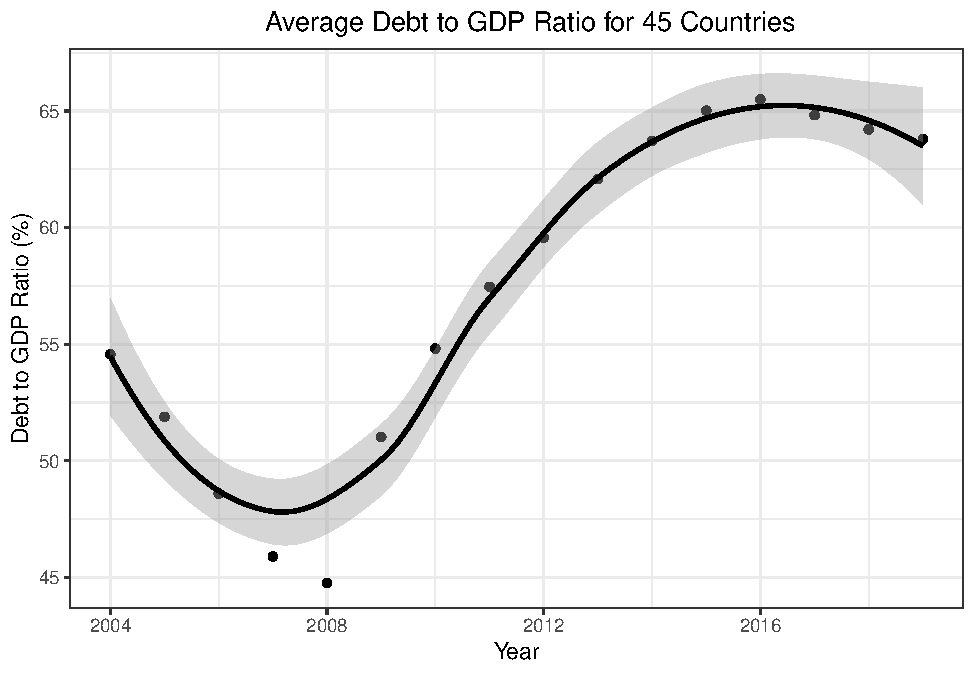
\includegraphics{final_project_files/figure-latex/unnamed-chunk-2-1.pdf}

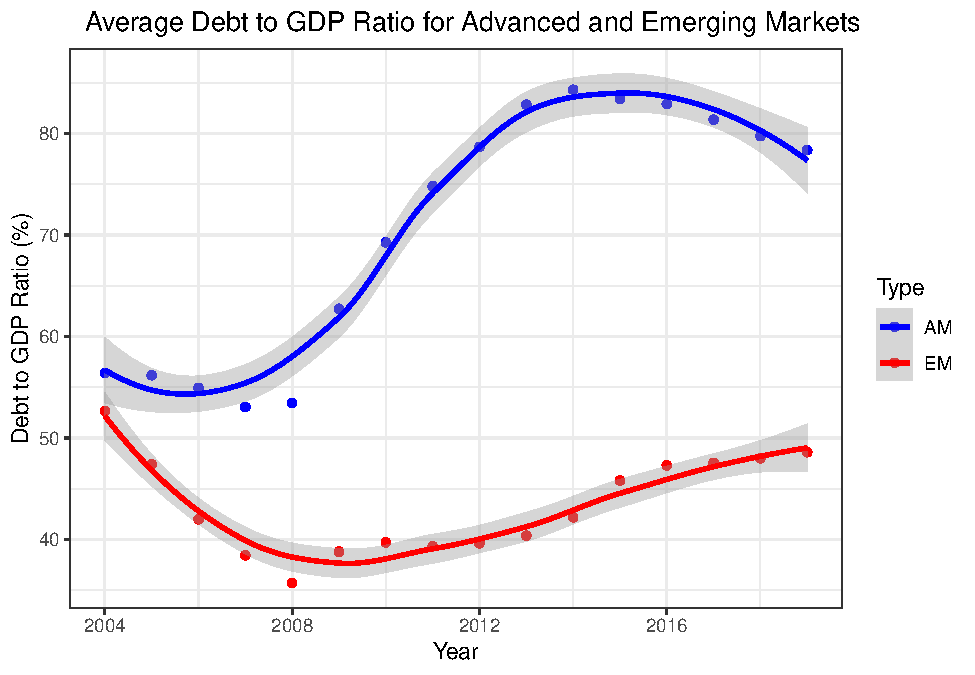
\includegraphics{final_project_files/figure-latex/unnamed-chunk-3-1.pdf}

\section{Stylized Facts}\label{stylized-facts}

Firstly, some stylized facts will be explained in relation to our
dataset.

\subsection{Countries have different indebtedness
levels}\label{countries-have-different-indebtedness-levels}

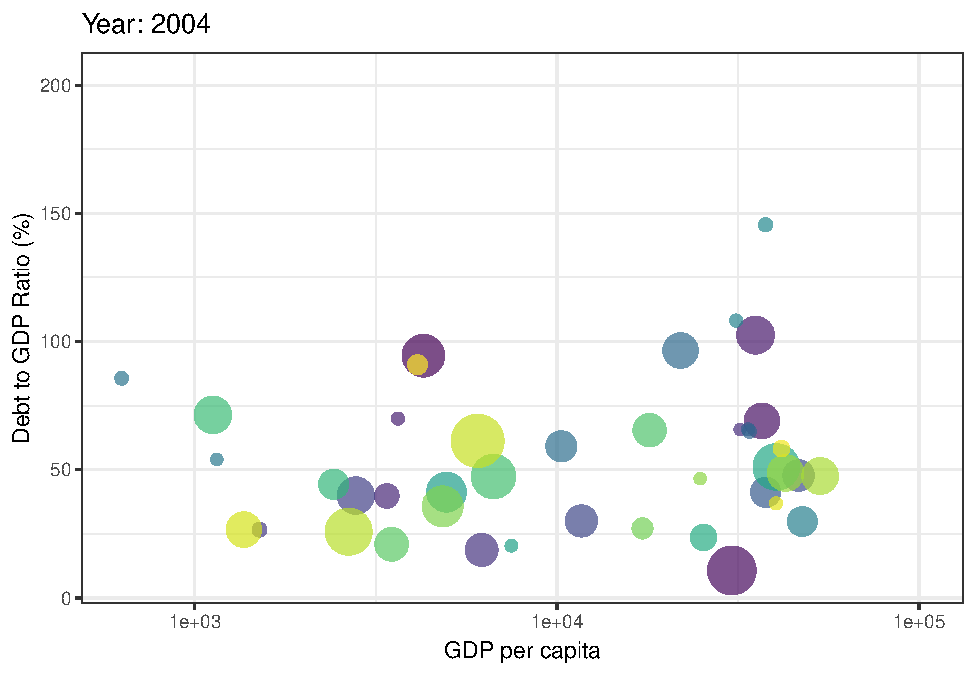
\includegraphics{final_project_files/figure-latex/unnamed-chunk-4-1.pdf}

As the map shown above makes clear, countries around the world have
contrasting levels of debt to GDP. Nations in grey are not part of our
sample.

\subsection{The level of indebtedness in the world has varied
considerably in recent
years}\label{the-level-of-indebtedness-in-the-world-has-varied-considerably-in-recent-years}

\includegraphics{final_project_files/figure-latex/unnamed-chunk-5-1.pdf}

It is possible to observe that the average indebtedness in the countries
fell a lot in 2008, rise until 2018 and has been showing a slight drop.

\subsection{Advanced markets are more indebted than emerging
markets}\label{advanced-markets-are-more-indebted-than-emerging-markets}

\includegraphics{final_project_files/figure-latex/unnamed-chunk-6-1.pdf}

\subsection{The relationship between debt and GDP is not
clear}\label{the-relationship-between-debt-and-gdp-is-not-clear}

\includegraphics{final_project_files/figure-latex/unnamed-chunk-7-1.pdf}

Even though advanced markets have a higher debt level than emerging
markets, the relationship between GDP per capita and debt to GDP ratio
is not clear.

\subsection{It is not possible to observe that countries with more than
90\% debt to GDP grow
less}\label{it-is-not-possible-to-observe-that-countries-with-more-than-90-debt-to-gdp-grow-less}

\includegraphics{final_project_files/figure-latex/unnamed-chunk-8-1.pdf}

Contrasting with Reinhart and Rogoff (2010), this dataset does not show
a clear pattern of decreasing GDP growth beyond the 90\% debt to GDP
level for advanced economies (marked in red).

\includegraphics{final_project_files/figure-latex/unnamed-chunk-9-1.pdf}

Concerning emerging economies, Reinhart et. al (2003) finds that real
growth might be constrained even with low levels of indebtedness - such
as 15 or 20\%. Once again, the selection of countries and time space
here goes in a different direction.

\subsection{Foreign investors have a preference for allocating their
resources in advanced
markets}\label{foreign-investors-have-a-preference-for-allocating-their-resources-in-advanced-markets}

\includegraphics{final_project_files/figure-latex/unnamed-chunk-10-1.pdf}

It is possible to observe that foreign investors have allocated much
more resources in bonds from advanced markets. In addition, we can see
that since 2012, the participation of foreign investors in government
bonds has accelerated.

\subsection{The participation of domestic investors in the composition
of debt it is not invariant over
time}\label{the-participation-of-domestic-investors-in-the-composition-of-debt-it-is-not-invariant-over-time}

\includegraphics{final_project_files/figure-latex/unnamed-chunk-11-1.pdf}

In addition to the domestic participation in debt varying for both
emerging and advanced countries, it is possible to infer that those
variations are inverse.

\subsection{There is no clear relationship between debt and
inflation}\label{there-is-no-clear-relationship-between-debt-and-inflation}

\includegraphics{final_project_files/figure-latex/unnamed-chunk-12-1.pdf}

\section{Econometrics}\label{econometrics}

\subsection{REG 1 (foreign menos BC)}\label{reg-1-foreign-menos-bc}

\begin{verbatim}
## Oneway (individual) effect Within Model
## 
## Call:
## plm(formula = for_ex_BC ~ debt_to_GDP_ + log(debt_to_GDP_) + 
##     log(debt_to_GDP_) + fx_ + GDP_per_cap_cte + inflation_mean + 
##     nominal_rate + vix_EUA + vix_EUR + taxes + develop + account_balance + 
##     lending_borrow + unemployment, data = panel_dataset)
## 
## Unbalanced Panel: n = 25, T = 1-16, N = 319
## 
## Residuals:
##       Min.    1st Qu.     Median    3rd Qu.       Max. 
## -0.1462935 -0.0308440  0.0013596  0.0319784  0.1292437 
## 
## Coefficients:
##                      Estimate  Std. Error t-value  Pr(>|t|)    
## debt_to_GDP_       3.4729e-05  5.4372e-04  0.0639 0.9491162    
## log(debt_to_GDP_)  4.1636e-02  2.1237e-02  1.9606 0.0509142 .  
## fx_               -7.4913e-02  4.2426e-02 -1.7657 0.0785250 .  
## GDP_per_cap_cte    1.6474e-06  1.2908e-06  1.2763 0.2029094    
## inflation_mean    -1.1094e-04  2.0609e-03 -0.0538 0.9571091    
## nominal_rate       1.2395e-03  1.2841e-03  0.9653 0.3352365    
## vix_EUA           -3.3978e-03  1.3051e-03 -2.6034 0.0097183 ** 
## vix_EUR            1.5876e-03  1.3184e-03  1.2042 0.2295189    
## taxes              3.8466e-03  1.1242e-03  3.4218 0.0007142 ***
## account_balance   -1.1980e-06  1.0552e-06 -1.1354 0.2571778    
## lending_borrow    -4.9637e-06  1.5878e-06 -3.1260 0.0019567 ** 
## unemployment      -3.8006e-06  2.4113e-06 -1.5762 0.1161100    
## ---
## Signif. codes:  0 '***' 0.001 '**' 0.01 '*' 0.05 '.' 0.1 ' ' 1
## 
## Total Sum of Squares:    0.8418
## Residual Sum of Squares: 0.64719
## R-Squared:      0.23118
## Adj. R-Squared: 0.13303
## F-statistic: 7.06617 on 12 and 282 DF, p-value: 3.065e-11
\end{verbatim}

\subsection{REG 1.1}\label{reg-1.1}

\begin{Shaded}
\begin{Highlighting}[]
\NormalTok{reg1.}\DecValTok{1}\NormalTok{ <-}\StringTok{ }\KeywordTok{plm}\NormalTok{(for_ex_BC }\OperatorTok{~}\StringTok{  }\KeywordTok{log}\NormalTok{(foreign_debt_) }\OperatorTok{+}\StringTok{ }\NormalTok{debt_to_GDP_ }\OperatorTok{+}\StringTok{ }\NormalTok{fx_ }\OperatorTok{+}\StringTok{ }\NormalTok{GDP_per_cap_cte }\OperatorTok{+}\StringTok{ }\NormalTok{nominal_rate }\OperatorTok{+}\StringTok{ }\NormalTok{continent }\OperatorTok{+}\StringTok{ }\NormalTok{vix_EUA }\OperatorTok{+}\StringTok{ }\NormalTok{vix_EUR }\OperatorTok{+}\StringTok{ }\NormalTok{taxes }\OperatorTok{+}\StringTok{ }\NormalTok{develop }\OperatorTok{+}\StringTok{ }\NormalTok{account_balance }\OperatorTok{+}\StringTok{ }\NormalTok{lending_borrow }\OperatorTok{+}\StringTok{ }\NormalTok{unemployment }\OperatorTok{+}\StringTok{ }\NormalTok{inflation_mean, }\DataTypeTok{data =}\NormalTok{ panel_dataset )}

\KeywordTok{summary}\NormalTok{(reg1.}\DecValTok{1}\NormalTok{)}
\end{Highlighting}
\end{Shaded}

\begin{verbatim}
## Oneway (individual) effect Within Model
## 
## Call:
## plm(formula = for_ex_BC ~ log(foreign_debt_) + debt_to_GDP_ + 
##     fx_ + GDP_per_cap_cte + nominal_rate + continent + vix_EUA + 
##     vix_EUR + taxes + develop + account_balance + lending_borrow + 
##     unemployment + inflation_mean, data = panel_dataset)
## 
## Unbalanced Panel: n = 25, T = 1-16, N = 319
## 
## Residuals:
##       Min.    1st Qu.     Median    3rd Qu.       Max. 
## -0.1205405 -0.0266137  0.0017047  0.0267820  0.1051343 
## 
## Coefficients:
##                       Estimate  Std. Error t-value  Pr(>|t|)    
## log(foreign_debt_)  6.6159e-02  7.0684e-03  9.3598 < 2.2e-16 ***
## debt_to_GDP_       -1.1448e-03  3.5575e-04 -3.2179 0.0014422 ** 
## fx_                -1.8300e-02  3.7553e-02 -0.4873 0.6264062    
## GDP_per_cap_cte     3.6651e-06  1.1565e-06  3.1692 0.0016966 ** 
## nominal_rate        7.7145e-04  1.1282e-03  0.6838 0.4946748    
## vix_EUA            -2.0954e-04  1.1998e-03 -0.1747 0.8614785    
## vix_EUR            -3.4267e-04  1.1767e-03 -0.2912 0.7711002    
## taxes               3.3462e-03  9.9007e-04  3.3798 0.0008277 ***
## account_balance    -1.1598e-06  9.1691e-07 -1.2649 0.2069625    
## lending_borrow     -5.3550e-07  1.4675e-06 -0.3649 0.7154611    
## unemployment        3.1301e-06  2.2533e-06  1.3891 0.1659046    
## inflation_mean     -2.0485e-03  1.8242e-03 -1.1230 0.2624106    
## ---
## Signif. codes:  0 '***' 0.001 '**' 0.01 '*' 0.05 '.' 0.1 ' ' 1
## 
## Total Sum of Squares:    0.8418
## Residual Sum of Squares: 0.50052
## R-Squared:      0.40541
## Adj. R-Squared: 0.32951
## F-statistic: 16.0232 on 12 and 282 DF, p-value: < 2.22e-16
\end{verbatim}

\subsection{REG 1.2}\label{reg-1.2}

\begin{Shaded}
\begin{Highlighting}[]
\NormalTok{reg1.}\DecValTok{2}\NormalTok{ <-}\StringTok{ }\KeywordTok{plm}\NormalTok{(for_ex_BC }\OperatorTok{~}\StringTok{ }\KeywordTok{log}\NormalTok{(foreign_debt_) }\OperatorTok{+}\StringTok{ }\NormalTok{debt_to_GDP_ }\OperatorTok{+}\StringTok{ }\NormalTok{fx_ }\OperatorTok{+}\StringTok{ }\NormalTok{GDP_per_cap_cte }\OperatorTok{+}\StringTok{ }\NormalTok{nominal_rate }\OperatorTok{+}\StringTok{ }\NormalTok{continent }\OperatorTok{+}\StringTok{ }\NormalTok{vix_EUA }\OperatorTok{+}\StringTok{ }\NormalTok{vix_EUR }\OperatorTok{+}\StringTok{ }\NormalTok{taxes }\OperatorTok{+}\StringTok{ }\NormalTok{develop }\OperatorTok{+}\StringTok{ }\NormalTok{account_balance }\OperatorTok{+}\StringTok{ }\NormalTok{lending_borrow }\OperatorTok{+}\StringTok{ }\NormalTok{unemployment }\OperatorTok{+}\StringTok{ }\NormalTok{inflation_mean, }\DataTypeTok{data =}\NormalTok{ panel_dataset )}

\KeywordTok{summary}\NormalTok{(reg1.}\DecValTok{2}\NormalTok{)}
\end{Highlighting}
\end{Shaded}

\begin{verbatim}
## Oneway (individual) effect Within Model
## 
## Call:
## plm(formula = for_ex_BC ~ log(foreign_debt_) + debt_to_GDP_ + 
##     fx_ + GDP_per_cap_cte + nominal_rate + continent + vix_EUA + 
##     vix_EUR + taxes + develop + account_balance + lending_borrow + 
##     unemployment + inflation_mean, data = panel_dataset)
## 
## Unbalanced Panel: n = 25, T = 1-16, N = 319
## 
## Residuals:
##       Min.    1st Qu.     Median    3rd Qu.       Max. 
## -0.1205405 -0.0266137  0.0017047  0.0267820  0.1051343 
## 
## Coefficients:
##                       Estimate  Std. Error t-value  Pr(>|t|)    
## log(foreign_debt_)  6.6159e-02  7.0684e-03  9.3598 < 2.2e-16 ***
## debt_to_GDP_       -1.1448e-03  3.5575e-04 -3.2179 0.0014422 ** 
## fx_                -1.8300e-02  3.7553e-02 -0.4873 0.6264062    
## GDP_per_cap_cte     3.6651e-06  1.1565e-06  3.1692 0.0016966 ** 
## nominal_rate        7.7145e-04  1.1282e-03  0.6838 0.4946748    
## vix_EUA            -2.0954e-04  1.1998e-03 -0.1747 0.8614785    
## vix_EUR            -3.4267e-04  1.1767e-03 -0.2912 0.7711002    
## taxes               3.3462e-03  9.9007e-04  3.3798 0.0008277 ***
## account_balance    -1.1598e-06  9.1691e-07 -1.2649 0.2069625    
## lending_borrow     -5.3550e-07  1.4675e-06 -0.3649 0.7154611    
## unemployment        3.1301e-06  2.2533e-06  1.3891 0.1659046    
## inflation_mean     -2.0485e-03  1.8242e-03 -1.1230 0.2624106    
## ---
## Signif. codes:  0 '***' 0.001 '**' 0.01 '*' 0.05 '.' 0.1 ' ' 1
## 
## Total Sum of Squares:    0.8418
## Residual Sum of Squares: 0.50052
## R-Squared:      0.40541
## Adj. R-Squared: 0.32951
## F-statistic: 16.0232 on 12 and 282 DF, p-value: < 2.22e-16
\end{verbatim}

\subsection{REG 1.3}\label{reg-1.3}

\begin{Shaded}
\begin{Highlighting}[]
\NormalTok{reg1.}\DecValTok{3}\NormalTok{ <-}\StringTok{ }\KeywordTok{plm}\NormalTok{(for_ex_BC }\OperatorTok{~}\StringTok{ }\NormalTok{debt_to_GDP_ }\OperatorTok{+}\StringTok{ }\NormalTok{fx_ }\OperatorTok{+}\StringTok{ }\NormalTok{GDP_per_cap_cte }\OperatorTok{+}\StringTok{ }\NormalTok{nominal_rate }\OperatorTok{+}\StringTok{ }\NormalTok{continent }\OperatorTok{+}\StringTok{ }\NormalTok{vix_EUA }\OperatorTok{+}\StringTok{ }\NormalTok{vix_EUR }\OperatorTok{+}\StringTok{ }\NormalTok{taxes }\OperatorTok{+}\StringTok{ }\NormalTok{develop }\OperatorTok{+}\StringTok{ }\NormalTok{account_balance }\OperatorTok{+}\StringTok{ }\NormalTok{lending_borrow }\OperatorTok{+}\StringTok{ }\NormalTok{unemployment }\OperatorTok{+}\StringTok{ }\NormalTok{inflation_mean, }\DataTypeTok{data =}\NormalTok{ panel_dataset )}

\KeywordTok{summary}\NormalTok{(reg1.}\DecValTok{3}\NormalTok{)}
\end{Highlighting}
\end{Shaded}

\begin{verbatim}
## Oneway (individual) effect Within Model
## 
## Call:
## plm(formula = for_ex_BC ~ debt_to_GDP_ + fx_ + GDP_per_cap_cte + 
##     nominal_rate + continent + vix_EUA + vix_EUR + taxes + develop + 
##     account_balance + lending_borrow + unemployment + inflation_mean, 
##     data = panel_dataset)
## 
## Unbalanced Panel: n = 25, T = 1-16, N = 319
## 
## Residuals:
##        Min.     1st Qu.      Median     3rd Qu.        Max. 
## -0.13959699 -0.02922251 -0.00044393  0.03456053  0.13006769 
## 
## Coefficients:
##                    Estimate  Std. Error t-value  Pr(>|t|)    
## debt_to_GDP_     8.9721e-04  3.2114e-04  2.7939 0.0055639 ** 
## fx_             -6.7892e-02  4.2487e-02 -1.5980 0.1111650    
## GDP_per_cap_cte  1.5756e-06  1.2968e-06  1.2150 0.2253709    
## nominal_rate     1.1040e-03  1.2887e-03  0.8567 0.3923479    
## vix_EUA         -3.5230e-03  1.3101e-03 -2.6891 0.0075891 ** 
## vix_EUR          1.5454e-03  1.3248e-03  1.1665 0.2444011    
## taxes            3.8503e-03  1.1298e-03  3.4079 0.0007496 ***
## account_balance -8.7295e-07  1.0473e-06 -0.8335 0.4052378    
## lending_borrow  -5.6502e-06  1.5565e-06 -3.6300 0.0003362 ***
## unemployment    -4.2660e-06  2.4116e-06 -1.7689 0.0779815 .  
## inflation_mean  -1.0769e-04  2.0712e-03 -0.0520 0.9585717    
## ---
## Signif. codes:  0 '***' 0.001 '**' 0.01 '*' 0.05 '.' 0.1 ' ' 1
## 
## Total Sum of Squares:    0.8418
## Residual Sum of Squares: 0.65602
## R-Squared:      0.2207
## Adj. R-Squared: 0.12432
## F-statistic: 7.2859 on 11 and 283 DF, p-value: 5.8955e-11
\end{verbatim}

\subsection{REG 1.4}\label{reg-1.4}

\begin{Shaded}
\begin{Highlighting}[]
\NormalTok{reg1.}\DecValTok{4}\NormalTok{ <-}\StringTok{ }\KeywordTok{plm}\NormalTok{(for_ex_BC }\OperatorTok{~}\StringTok{ }\NormalTok{debt_to_GDP_ }\OperatorTok{+}\StringTok{ }\NormalTok{fx_ }\OperatorTok{+}\StringTok{ }\NormalTok{GDP_per_cap_cte }\OperatorTok{+}\StringTok{ }\NormalTok{nominal_rate }\OperatorTok{+}\StringTok{ }\NormalTok{continent }\OperatorTok{+}\StringTok{ }\NormalTok{vix_EUA }\OperatorTok{+}\StringTok{ }\NormalTok{vix_EUR }\OperatorTok{+}\StringTok{ }\NormalTok{taxes }\OperatorTok{+}\StringTok{ }\NormalTok{develop }\OperatorTok{+}\StringTok{ }\NormalTok{account_balance }\OperatorTok{+}\StringTok{ }\NormalTok{lending_borrow }\OperatorTok{+}\StringTok{ }\NormalTok{unemployment }\OperatorTok{+}\StringTok{ }\NormalTok{inflation_mean, }\DataTypeTok{data =}\NormalTok{ panel_dataset )}

\KeywordTok{summary}\NormalTok{(reg1.}\DecValTok{4}\NormalTok{)}
\end{Highlighting}
\end{Shaded}

\begin{verbatim}
## Oneway (individual) effect Within Model
## 
## Call:
## plm(formula = for_ex_BC ~ debt_to_GDP_ + fx_ + GDP_per_cap_cte + 
##     nominal_rate + continent + vix_EUA + vix_EUR + taxes + develop + 
##     account_balance + lending_borrow + unemployment + inflation_mean, 
##     data = panel_dataset)
## 
## Unbalanced Panel: n = 25, T = 1-16, N = 319
## 
## Residuals:
##        Min.     1st Qu.      Median     3rd Qu.        Max. 
## -0.13959699 -0.02922251 -0.00044393  0.03456053  0.13006769 
## 
## Coefficients:
##                    Estimate  Std. Error t-value  Pr(>|t|)    
## debt_to_GDP_     8.9721e-04  3.2114e-04  2.7939 0.0055639 ** 
## fx_             -6.7892e-02  4.2487e-02 -1.5980 0.1111650    
## GDP_per_cap_cte  1.5756e-06  1.2968e-06  1.2150 0.2253709    
## nominal_rate     1.1040e-03  1.2887e-03  0.8567 0.3923479    
## vix_EUA         -3.5230e-03  1.3101e-03 -2.6891 0.0075891 ** 
## vix_EUR          1.5454e-03  1.3248e-03  1.1665 0.2444011    
## taxes            3.8503e-03  1.1298e-03  3.4079 0.0007496 ***
## account_balance -8.7295e-07  1.0473e-06 -0.8335 0.4052378    
## lending_borrow  -5.6502e-06  1.5565e-06 -3.6300 0.0003362 ***
## unemployment    -4.2660e-06  2.4116e-06 -1.7689 0.0779815 .  
## inflation_mean  -1.0769e-04  2.0712e-03 -0.0520 0.9585717    
## ---
## Signif. codes:  0 '***' 0.001 '**' 0.01 '*' 0.05 '.' 0.1 ' ' 1
## 
## Total Sum of Squares:    0.8418
## Residual Sum of Squares: 0.65602
## R-Squared:      0.2207
## Adj. R-Squared: 0.12432
## F-statistic: 7.2859 on 11 and 283 DF, p-value: 5.8955e-11
\end{verbatim}

\subsection{REG 1.5}\label{reg-1.5}

\begin{Shaded}
\begin{Highlighting}[]
\NormalTok{reg1.}\DecValTok{5}\NormalTok{ <-}\StringTok{ }\KeywordTok{plm}\NormalTok{(for_ex_BC }\OperatorTok{~}\StringTok{ }\KeywordTok{log}\NormalTok{(foreign_debt_) }\OperatorTok{+}\StringTok{ }\NormalTok{debt_to_GDP_ }\OperatorTok{+}\StringTok{ }\NormalTok{GDP_per_cap_cte }\OperatorTok{+}\StringTok{ }\NormalTok{nominal_rate }\OperatorTok{+}\StringTok{ }\NormalTok{continent }\OperatorTok{+}\StringTok{ }\NormalTok{vix_EUA }\OperatorTok{+}\StringTok{ }\NormalTok{vix_EUR }\OperatorTok{+}\StringTok{ }\NormalTok{taxes }\OperatorTok{+}\StringTok{ }\NormalTok{develop }\OperatorTok{+}\StringTok{ }\NormalTok{account_balance }\OperatorTok{+}\StringTok{ }\NormalTok{lending_borrow }\OperatorTok{+}\StringTok{ }\NormalTok{unemployment }\OperatorTok{+}\StringTok{ }\NormalTok{inflation_mean, }\DataTypeTok{data =}\NormalTok{ panel_dataset )}

\KeywordTok{summary}\NormalTok{(reg1.}\DecValTok{5}\NormalTok{)}
\end{Highlighting}
\end{Shaded}

\begin{verbatim}
## Oneway (individual) effect Within Model
## 
## Call:
## plm(formula = for_ex_BC ~ log(foreign_debt_) + debt_to_GDP_ + 
##     GDP_per_cap_cte + nominal_rate + continent + vix_EUA + vix_EUR + 
##     taxes + develop + account_balance + lending_borrow + unemployment + 
##     inflation_mean, data = panel_dataset)
## 
## Unbalanced Panel: n = 25, T = 1-16, N = 319
## 
## Residuals:
##       Min.    1st Qu.     Median    3rd Qu.       Max. 
## -0.1203042 -0.0269057  0.0018461  0.0265785  0.1047314 
## 
## Coefficients:
##                       Estimate  Std. Error t-value  Pr(>|t|)    
## log(foreign_debt_)  6.6645e-02  6.9883e-03  9.5367 < 2.2e-16 ***
## debt_to_GDP_       -1.1297e-03  3.5392e-04 -3.1918 0.0015729 ** 
## GDP_per_cap_cte     3.5987e-06  1.1469e-06  3.1379 0.0018814 ** 
## nominal_rate        7.8718e-04  1.1262e-03  0.6989 0.4851583    
## vix_EUA            -2.2690e-04  1.1976e-03 -0.1895 0.8498697    
## vix_EUR            -3.6414e-04  1.1743e-03 -0.3101 0.7567149    
## taxes               3.2943e-03  9.8300e-04  3.3513 0.0009137 ***
## account_balance    -1.1235e-06  9.1264e-07 -1.2310 0.2193487    
## lending_borrow     -5.0915e-07  1.4646e-06 -0.3476 0.7283641    
## unemployment        3.1547e-06  2.2497e-06  1.4022 0.1619415    
## inflation_mean     -1.9583e-03  1.8123e-03 -1.0805 0.2808304    
## ---
## Signif. codes:  0 '***' 0.001 '**' 0.01 '*' 0.05 '.' 0.1 ' ' 1
## 
## Total Sum of Squares:    0.8418
## Residual Sum of Squares: 0.50094
## R-Squared:      0.40491
## Adj. R-Squared: 0.33131
## F-statistic: 17.5054 on 11 and 283 DF, p-value: < 2.22e-16
\end{verbatim}

\subsection{REG 1.6}\label{reg-1.6}

\begin{Shaded}
\begin{Highlighting}[]
\NormalTok{reg1.}\DecValTok{6}\NormalTok{ <-}\StringTok{ }\KeywordTok{plm}\NormalTok{(for_ex_BC }\OperatorTok{~}\StringTok{ }\KeywordTok{log}\NormalTok{(foreign_debt_) }\OperatorTok{+}\StringTok{ }\NormalTok{debt_to_GDP_ }\OperatorTok{+}\StringTok{ }\NormalTok{fx_ }\OperatorTok{+}\StringTok{ }\NormalTok{nominal_rate }\OperatorTok{+}\StringTok{ }\NormalTok{continent }\OperatorTok{+}\StringTok{ }\NormalTok{vix_EUA }\OperatorTok{+}\StringTok{ }\NormalTok{vix_EUR }\OperatorTok{+}\StringTok{ }\NormalTok{taxes }\OperatorTok{+}\StringTok{ }\NormalTok{develop }\OperatorTok{+}\StringTok{ }\NormalTok{account_balance }\OperatorTok{+}\StringTok{ }\NormalTok{lending_borrow }\OperatorTok{+}\StringTok{ }\NormalTok{unemployment }\OperatorTok{+}\StringTok{ }\NormalTok{inflation_mean, }\DataTypeTok{data =}\NormalTok{ panel_dataset )}

\KeywordTok{summary}\NormalTok{(reg1.}\DecValTok{6}\NormalTok{)}
\end{Highlighting}
\end{Shaded}

\begin{verbatim}
## Oneway (individual) effect Within Model
## 
## Call:
## plm(formula = for_ex_BC ~ log(foreign_debt_) + debt_to_GDP_ + 
##     fx_ + nominal_rate + continent + vix_EUA + vix_EUR + taxes + 
##     develop + account_balance + lending_borrow + unemployment + 
##     inflation_mean, data = panel_dataset)
## 
## Unbalanced Panel: n = 25, T = 1-16, N = 319
## 
## Residuals:
##       Min.    1st Qu.     Median    3rd Qu.       Max. 
## -0.1269907 -0.0270644  0.0038991  0.0263459  0.1030628 
## 
## Coefficients:
##                       Estimate  Std. Error t-value  Pr(>|t|)    
## log(foreign_debt_)  6.1835e-02  7.0454e-03  8.7766 < 2.2e-16 ***
## debt_to_GDP_       -1.0296e-03  3.5950e-04 -2.8641  0.004496 ** 
## fx_                -4.2819e-03  3.7883e-02 -0.1130  0.910087    
## nominal_rate        4.9009e-04  1.1425e-03  0.4289  0.668290    
## vix_EUA            -9.0953e-04  1.1980e-03 -0.7592  0.448346    
## vix_EUR            -1.8621e-04  1.1943e-03 -0.1559  0.876212    
## taxes               2.9624e-03  9.9821e-04  2.9677  0.003257 ** 
## account_balance    -1.5337e-06  9.2370e-07 -1.6604  0.097932 .  
## lending_borrow      8.2171e-07  1.4259e-06  0.5763  0.564893    
## unemployment        3.1284e-06  2.2891e-06  1.3667  0.172808    
## inflation_mean     -1.7151e-03  1.8500e-03 -0.9271  0.354670    
## ---
## Signif. codes:  0 '***' 0.001 '**' 0.01 '*' 0.05 '.' 0.1 ' ' 1
## 
## Total Sum of Squares:    0.8418
## Residual Sum of Squares: 0.51835
## R-Squared:      0.38423
## Adj. R-Squared: 0.30808
## F-statistic: 16.0537 on 11 and 283 DF, p-value: < 2.22e-16
\end{verbatim}

\subsection{REG 1.7}\label{reg-1.7}

\begin{Shaded}
\begin{Highlighting}[]
\NormalTok{reg1.}\DecValTok{7}\NormalTok{ <-}\StringTok{ }\KeywordTok{plm}\NormalTok{(for_ex_BC }\OperatorTok{~}\StringTok{ }\KeywordTok{log}\NormalTok{(foreign_debt_) }\OperatorTok{+}\StringTok{ }\NormalTok{debt_to_GDP_ }\OperatorTok{+}\StringTok{ }\NormalTok{fx_ }\OperatorTok{+}\StringTok{ }\NormalTok{GDP_per_cap_cte }\OperatorTok{+}\StringTok{ }\NormalTok{continent }\OperatorTok{+}\StringTok{ }\NormalTok{vix_EUA }\OperatorTok{+}\StringTok{ }\NormalTok{vix_EUR }\OperatorTok{+}\StringTok{ }\NormalTok{taxes }\OperatorTok{+}\StringTok{ }\NormalTok{develop }\OperatorTok{+}\StringTok{ }\NormalTok{account_balance }\OperatorTok{+}\StringTok{ }\NormalTok{lending_borrow }\OperatorTok{+}\StringTok{ }\NormalTok{unemployment }\OperatorTok{+}\StringTok{ }\NormalTok{inflation_mean, }\DataTypeTok{data =}\NormalTok{ panel_dataset )}

\KeywordTok{summary}\NormalTok{(reg1.}\DecValTok{7}\NormalTok{)}
\end{Highlighting}
\end{Shaded}

\begin{verbatim}
## Oneway (individual) effect Within Model
## 
## Call:
## plm(formula = for_ex_BC ~ log(foreign_debt_) + debt_to_GDP_ + 
##     fx_ + GDP_per_cap_cte + continent + vix_EUA + vix_EUR + taxes + 
##     develop + account_balance + lending_borrow + unemployment + 
##     inflation_mean, data = panel_dataset)
## 
## Unbalanced Panel: n = 41, T = 7-16, N = 588
## 
## Residuals:
##       Min.    1st Qu.     Median    3rd Qu.       Max. 
## -0.1873919 -0.0382907  0.0010503  0.0364233  0.2252027 
## 
## Coefficients:
##                       Estimate  Std. Error t-value  Pr(>|t|)    
## log(foreign_debt_)  7.4179e-02  7.8077e-03  9.5007 < 2.2e-16 ***
## debt_to_GDP_       -2.6011e-03  3.2402e-04 -8.0276 6.326e-15 ***
## fx_                 8.9594e-02  3.6032e-02  2.4865   0.01320 *  
## GDP_per_cap_cte     2.1089e-06  1.0699e-06  1.9712   0.04921 *  
## vix_EUA            -8.0181e-04  1.2631e-03 -0.6348   0.52584    
## vix_EUR            -2.5829e-04  1.2256e-03 -0.2107   0.83317    
## taxes              -9.6997e-04  1.1096e-03 -0.8742   0.38242    
## account_balance    -7.9719e-07  9.2258e-07 -0.8641   0.38793    
## lending_borrow     -5.1073e-06  1.2114e-06 -4.2160 2.919e-05 ***
## unemployment       -6.8815e-06  1.6409e-06 -4.1938 3.209e-05 ***
## inflation_mean      7.0189e-04  1.0269e-03  0.6835   0.49457    
## ---
## Signif. codes:  0 '***' 0.001 '**' 0.01 '*' 0.05 '.' 0.1 ' ' 1
## 
## Total Sum of Squares:    3.2407
## Residual Sum of Squares: 2.0475
## R-Squared:      0.36819
## Adj. R-Squared: 0.30807
## F-statistic: 28.3961 on 11 and 536 DF, p-value: < 2.22e-16
\end{verbatim}

\subsection{REG 1.8}\label{reg-1.8}

\begin{Shaded}
\begin{Highlighting}[]
\NormalTok{reg1.}\DecValTok{8}\NormalTok{ <-}\StringTok{ }\KeywordTok{plm}\NormalTok{(for_ex_BC }\OperatorTok{~}\StringTok{  }\KeywordTok{log}\NormalTok{(foreign_debt_) }\OperatorTok{+}\StringTok{ }\NormalTok{debt_to_GDP_ }\OperatorTok{+}\StringTok{ }\NormalTok{fx_ }\OperatorTok{+}\StringTok{ }\NormalTok{GDP_per_cap_cte }\OperatorTok{+}\StringTok{ }\NormalTok{nominal_rate }\OperatorTok{+}\StringTok{ }\NormalTok{vix_EUA }\OperatorTok{+}\StringTok{ }\NormalTok{vix_EUR }\OperatorTok{+}\StringTok{ }\NormalTok{taxes }\OperatorTok{+}\StringTok{ }\NormalTok{develop }\OperatorTok{+}\StringTok{ }\NormalTok{account_balance }\OperatorTok{+}\StringTok{ }\NormalTok{lending_borrow }\OperatorTok{+}\StringTok{ }\NormalTok{unemployment }\OperatorTok{+}\StringTok{ }\NormalTok{inflation_mean, }\DataTypeTok{data =}\NormalTok{ panel_dataset )}

\KeywordTok{summary}\NormalTok{(reg1.}\DecValTok{8}\NormalTok{)}
\end{Highlighting}
\end{Shaded}

\begin{verbatim}
## Oneway (individual) effect Within Model
## 
## Call:
## plm(formula = for_ex_BC ~ log(foreign_debt_) + debt_to_GDP_ + 
##     fx_ + GDP_per_cap_cte + nominal_rate + vix_EUA + vix_EUR + 
##     taxes + develop + account_balance + lending_borrow + unemployment + 
##     inflation_mean, data = panel_dataset)
## 
## Unbalanced Panel: n = 25, T = 1-16, N = 319
## 
## Residuals:
##       Min.    1st Qu.     Median    3rd Qu.       Max. 
## -0.1205405 -0.0266137  0.0017047  0.0267820  0.1051343 
## 
## Coefficients:
##                       Estimate  Std. Error t-value  Pr(>|t|)    
## log(foreign_debt_)  6.6159e-02  7.0684e-03  9.3598 < 2.2e-16 ***
## debt_to_GDP_       -1.1448e-03  3.5575e-04 -3.2179 0.0014422 ** 
## fx_                -1.8300e-02  3.7553e-02 -0.4873 0.6264062    
## GDP_per_cap_cte     3.6651e-06  1.1565e-06  3.1692 0.0016966 ** 
## nominal_rate        7.7145e-04  1.1282e-03  0.6838 0.4946748    
## vix_EUA            -2.0954e-04  1.1998e-03 -0.1747 0.8614785    
## vix_EUR            -3.4267e-04  1.1767e-03 -0.2912 0.7711002    
## taxes               3.3462e-03  9.9007e-04  3.3798 0.0008277 ***
## account_balance    -1.1598e-06  9.1691e-07 -1.2649 0.2069625    
## lending_borrow     -5.3550e-07  1.4675e-06 -0.3649 0.7154611    
## unemployment        3.1301e-06  2.2533e-06  1.3891 0.1659046    
## inflation_mean     -2.0485e-03  1.8242e-03 -1.1230 0.2624106    
## ---
## Signif. codes:  0 '***' 0.001 '**' 0.01 '*' 0.05 '.' 0.1 ' ' 1
## 
## Total Sum of Squares:    0.8418
## Residual Sum of Squares: 0.50052
## R-Squared:      0.40541
## Adj. R-Squared: 0.32951
## F-statistic: 16.0232 on 12 and 282 DF, p-value: < 2.22e-16
\end{verbatim}

\subsection{REG 1.9}\label{reg-1.9}

\begin{Shaded}
\begin{Highlighting}[]
\NormalTok{reg1.}\DecValTok{9}\NormalTok{ <-}\StringTok{ }\KeywordTok{plm}\NormalTok{(for_ex_BC }\OperatorTok{~}\StringTok{  }\KeywordTok{log}\NormalTok{(foreign_debt_) }\OperatorTok{+}\StringTok{ }\NormalTok{debt_to_GDP_ }\OperatorTok{+}\StringTok{ }\NormalTok{fx_ }\OperatorTok{+}\StringTok{ }\NormalTok{GDP_per_cap_cte }\OperatorTok{+}\StringTok{ }\NormalTok{nominal_rate }\OperatorTok{+}\StringTok{ }\NormalTok{continent }\OperatorTok{+}\StringTok{ }\NormalTok{vix_EUA }\OperatorTok{+}\StringTok{ }\NormalTok{taxes }\OperatorTok{+}\StringTok{ }\NormalTok{develop }\OperatorTok{+}\StringTok{ }\NormalTok{account_balance }\OperatorTok{+}\StringTok{ }\NormalTok{lending_borrow }\OperatorTok{+}\StringTok{ }\NormalTok{unemployment }\OperatorTok{+}\StringTok{ }\NormalTok{inflation_mean, }\DataTypeTok{data =}\NormalTok{ panel_dataset )}

\KeywordTok{summary}\NormalTok{(reg1.}\DecValTok{9}\NormalTok{)}
\end{Highlighting}
\end{Shaded}

\begin{verbatim}
## Oneway (individual) effect Within Model
## 
## Call:
## plm(formula = for_ex_BC ~ log(foreign_debt_) + debt_to_GDP_ + 
##     fx_ + GDP_per_cap_cte + nominal_rate + continent + vix_EUA + 
##     taxes + develop + account_balance + lending_borrow + unemployment + 
##     inflation_mean, data = panel_dataset)
## 
## Unbalanced Panel: n = 25, T = 1-16, N = 319
## 
## Residuals:
##       Min.    1st Qu.     Median    3rd Qu.       Max. 
## -0.1203699 -0.0265807  0.0012446  0.0271036  0.1052693 
## 
## Coefficients:
##                       Estimate  Std. Error t-value  Pr(>|t|)    
## log(foreign_debt_)  6.5806e-02  6.9525e-03  9.4651 < 2.2e-16 ***
## debt_to_GDP_       -1.1388e-03  3.5460e-04 -3.2117 0.0014720 ** 
## fx_                -1.8710e-02  3.7466e-02 -0.4994 0.6178947    
## GDP_per_cap_cte     3.6510e-06  1.1536e-06  3.1649 0.0017204 ** 
## nominal_rate        7.9942e-04  1.1223e-03  0.7123 0.4768605    
## vix_EUA            -5.3127e-04  4.6718e-04 -1.1372 0.2564302    
## taxes               3.3637e-03  9.8665e-04  3.4093 0.0007461 ***
## account_balance    -1.1516e-06  9.1499e-07 -1.2586 0.2092295    
## lending_borrow     -4.8397e-07  1.4545e-06 -0.3327 0.7395738    
## unemployment        3.1267e-06  2.2497e-06  1.3898 0.1656671    
## inflation_mean     -1.9984e-03  1.8131e-03 -1.1022 0.2713140    
## ---
## Signif. codes:  0 '***' 0.001 '**' 0.01 '*' 0.05 '.' 0.1 ' ' 1
## 
## Total Sum of Squares:    0.8418
## Residual Sum of Squares: 0.50067
## R-Squared:      0.40523
## Adj. R-Squared: 0.33168
## F-statistic: 17.5288 on 11 and 283 DF, p-value: < 2.22e-16
\end{verbatim}

\subsection{REG 1.10}\label{reg-1.10}

\begin{Shaded}
\begin{Highlighting}[]
\NormalTok{reg1.}\DecValTok{10}\NormalTok{ <-}\StringTok{ }\KeywordTok{plm}\NormalTok{(for_ex_BC }\OperatorTok{~}\StringTok{ }\KeywordTok{log}\NormalTok{(foreign_debt_) }\OperatorTok{+}\StringTok{ }\NormalTok{debt_to_GDP_ }\OperatorTok{+}\StringTok{ }\NormalTok{fx_ }\OperatorTok{+}\StringTok{ }\NormalTok{GDP_per_cap_cte }\OperatorTok{+}\StringTok{ }\NormalTok{nominal_rate }\OperatorTok{+}\StringTok{ }\NormalTok{continent }\OperatorTok{+}\StringTok{ }\NormalTok{vix_EUR }\OperatorTok{+}\StringTok{ }\NormalTok{taxes }\OperatorTok{+}\StringTok{ }\NormalTok{develop }\OperatorTok{+}\StringTok{ }\NormalTok{account_balance }\OperatorTok{+}\StringTok{ }\NormalTok{lending_borrow }\OperatorTok{+}\StringTok{ }\NormalTok{unemployment }\OperatorTok{+}\StringTok{ }\NormalTok{inflation_mean, }\DataTypeTok{data =}\NormalTok{ panel_dataset )}

\KeywordTok{summary}\NormalTok{(reg1.}\DecValTok{10}\NormalTok{)}
\end{Highlighting}
\end{Shaded}

\begin{verbatim}
## Oneway (individual) effect Within Model
## 
## Call:
## plm(formula = for_ex_BC ~ log(foreign_debt_) + debt_to_GDP_ + 
##     fx_ + GDP_per_cap_cte + nominal_rate + continent + vix_EUR + 
##     taxes + develop + account_balance + lending_borrow + unemployment + 
##     inflation_mean, data = panel_dataset)
## 
## Unbalanced Panel: n = 25, T = 1-16, N = 319
## 
## Residuals:
##       Min.    1st Qu.     Median    3rd Qu.       Max. 
## -0.1203785 -0.0265729  0.0016909  0.0263529  0.1052203 
## 
## Coefficients:
##                       Estimate  Std. Error t-value  Pr(>|t|)    
## log(foreign_debt_)  6.6523e-02  6.7421e-03  9.8668 < 2.2e-16 ***
## debt_to_GDP_       -1.1485e-03  3.5449e-04 -3.2400 0.0013379 ** 
## fx_                -1.8495e-02  3.7472e-02 -0.4936 0.6219900    
## GDP_per_cap_cte     3.7023e-06  1.1348e-06  3.2626 0.0012391 ** 
## nominal_rate        7.6849e-04  1.1262e-03  0.6824 0.4955430    
## vix_EUR            -5.3191e-04  4.5815e-04 -1.1610 0.2466259    
## taxes               3.3369e-03  9.8693e-04  3.3811 0.0008236 ***
## account_balance    -1.1656e-06  9.1473e-07 -1.2742 0.2036302    
## lending_borrow     -5.4546e-07  1.4639e-06 -0.3726 0.7097226    
## unemployment        3.1312e-06  2.2495e-06  1.3920 0.1650232    
## inflation_mean     -2.1052e-03  1.7920e-03 -1.1748 0.2410590    
## ---
## Signif. codes:  0 '***' 0.001 '**' 0.01 '*' 0.05 '.' 0.1 ' ' 1
## 
## Total Sum of Squares:    0.8418
## Residual Sum of Squares: 0.50058
## R-Squared:      0.40535
## Adj. R-Squared: 0.3318
## F-statistic: 17.5371 on 11 and 283 DF, p-value: < 2.22e-16
\end{verbatim}

\subsection{REG 1.11}\label{reg-1.11}

\begin{Shaded}
\begin{Highlighting}[]
\NormalTok{reg1.}\DecValTok{11}\NormalTok{ <-}\StringTok{ }\KeywordTok{plm}\NormalTok{(for_ex_BC }\OperatorTok{~}\StringTok{  }\KeywordTok{log}\NormalTok{(foreign_debt_) }\OperatorTok{+}\StringTok{ }\NormalTok{debt_to_GDP_ }\OperatorTok{+}\StringTok{ }\NormalTok{fx_ }\OperatorTok{+}\StringTok{ }\NormalTok{GDP_per_cap_cte }\OperatorTok{+}\StringTok{ }\NormalTok{nominal_rate }\OperatorTok{+}\StringTok{ }\NormalTok{continent }\OperatorTok{+}\StringTok{ }\NormalTok{vix_EUA }\OperatorTok{+}\StringTok{ }\NormalTok{vix_EUR }\OperatorTok{+}\StringTok{ }\NormalTok{develop }\OperatorTok{+}\StringTok{ }\NormalTok{account_balance }\OperatorTok{+}\StringTok{ }\NormalTok{lending_borrow }\OperatorTok{+}\StringTok{ }\NormalTok{unemployment }\OperatorTok{+}\StringTok{ }\NormalTok{inflation_mean, }\DataTypeTok{data =}\NormalTok{ panel_dataset )}

\KeywordTok{summary}\NormalTok{(reg1.}\DecValTok{11}\NormalTok{)}
\end{Highlighting}
\end{Shaded}

\begin{verbatim}
## Oneway (individual) effect Within Model
## 
## Call:
## plm(formula = for_ex_BC ~ log(foreign_debt_) + debt_to_GDP_ + 
##     fx_ + GDP_per_cap_cte + nominal_rate + continent + vix_EUA + 
##     vix_EUR + develop + account_balance + lending_borrow + unemployment + 
##     inflation_mean, data = panel_dataset)
## 
## Unbalanced Panel: n = 25, T = 1-16, N = 348
## 
## Residuals:
##       Min.    1st Qu.     Median    3rd Qu.       Max. 
## -0.1215185 -0.0298425  0.0041748  0.0292424  0.1043434 
## 
## Coefficients:
##                       Estimate  Std. Error t-value  Pr(>|t|)    
## log(foreign_debt_)  7.6639e-02  6.4986e-03 11.7932 < 2.2e-16 ***
## debt_to_GDP_       -1.5595e-03  3.2726e-04 -4.7653 2.896e-06 ***
## fx_                -1.2500e-02  3.5642e-02 -0.3507  0.726055    
## GDP_per_cap_cte     3.3747e-06  1.1789e-06  2.8626  0.004486 ** 
## nominal_rate        8.4551e-04  1.0384e-03  0.8143  0.416109    
## vix_EUA             2.5967e-04  1.1251e-03  0.2308  0.817626    
## vix_EUR            -4.7441e-04  1.0880e-03 -0.4360  0.663109    
## account_balance    -2.0338e-06  8.8068e-07 -2.3094  0.021575 *  
## lending_borrow      1.1108e-06  1.4214e-06  0.7815  0.435098    
## unemployment        4.0242e-06  2.1295e-06  1.8898  0.059717 .  
## inflation_mean     -3.5882e-03  1.4403e-03 -2.4913  0.013248 *  
## ---
## Signif. codes:  0 '***' 0.001 '**' 0.01 '*' 0.05 '.' 0.1 ' ' 1
## 
## Total Sum of Squares:    1.064
## Residual Sum of Squares: 0.60691
## R-Squared:      0.42957
## Adj. R-Squared: 0.36558
## F-statistic: 21.3595 on 11 and 312 DF, p-value: < 2.22e-16
\end{verbatim}

\subsection{REG 1.12}\label{reg-1.12}

\begin{Shaded}
\begin{Highlighting}[]
\NormalTok{reg1.}\DecValTok{12}\NormalTok{ <-}\StringTok{ }\KeywordTok{plm}\NormalTok{(for_ex_BC }\OperatorTok{~}\StringTok{ }\KeywordTok{log}\NormalTok{(foreign_debt_) }\OperatorTok{+}\StringTok{ }\NormalTok{debt_to_GDP_ }\OperatorTok{+}\StringTok{ }\NormalTok{fx_ }\OperatorTok{+}\StringTok{ }\NormalTok{GDP_per_cap_cte }\OperatorTok{+}\StringTok{ }\NormalTok{nominal_rate }\OperatorTok{+}\StringTok{ }\NormalTok{continent }\OperatorTok{+}\StringTok{ }\NormalTok{vix_EUA }\OperatorTok{+}\StringTok{ }\NormalTok{vix_EUR }\OperatorTok{+}\StringTok{ }\NormalTok{taxes }\OperatorTok{+}\StringTok{ }\NormalTok{account_balance }\OperatorTok{+}\StringTok{ }\NormalTok{lending_borrow }\OperatorTok{+}\StringTok{ }\NormalTok{unemployment }\OperatorTok{+}\StringTok{ }\NormalTok{inflation_mean, }\DataTypeTok{data =}\NormalTok{ panel_dataset )}

\KeywordTok{summary}\NormalTok{(reg1.}\DecValTok{12}\NormalTok{)}
\end{Highlighting}
\end{Shaded}

\begin{verbatim}
## Oneway (individual) effect Within Model
## 
## Call:
## plm(formula = for_ex_BC ~ log(foreign_debt_) + debt_to_GDP_ + 
##     fx_ + GDP_per_cap_cte + nominal_rate + continent + vix_EUA + 
##     vix_EUR + taxes + account_balance + lending_borrow + unemployment + 
##     inflation_mean, data = panel_dataset)
## 
## Unbalanced Panel: n = 25, T = 1-16, N = 319
## 
## Residuals:
##       Min.    1st Qu.     Median    3rd Qu.       Max. 
## -0.1205405 -0.0266137  0.0017047  0.0267820  0.1051343 
## 
## Coefficients:
##                       Estimate  Std. Error t-value  Pr(>|t|)    
## log(foreign_debt_)  6.6159e-02  7.0684e-03  9.3598 < 2.2e-16 ***
## debt_to_GDP_       -1.1448e-03  3.5575e-04 -3.2179 0.0014422 ** 
## fx_                -1.8300e-02  3.7553e-02 -0.4873 0.6264062    
## GDP_per_cap_cte     3.6651e-06  1.1565e-06  3.1692 0.0016966 ** 
## nominal_rate        7.7145e-04  1.1282e-03  0.6838 0.4946748    
## vix_EUA            -2.0954e-04  1.1998e-03 -0.1747 0.8614785    
## vix_EUR            -3.4267e-04  1.1767e-03 -0.2912 0.7711002    
## taxes               3.3462e-03  9.9007e-04  3.3798 0.0008277 ***
## account_balance    -1.1598e-06  9.1691e-07 -1.2649 0.2069625    
## lending_borrow     -5.3550e-07  1.4675e-06 -0.3649 0.7154611    
## unemployment        3.1301e-06  2.2533e-06  1.3891 0.1659046    
## inflation_mean     -2.0485e-03  1.8242e-03 -1.1230 0.2624106    
## ---
## Signif. codes:  0 '***' 0.001 '**' 0.01 '*' 0.05 '.' 0.1 ' ' 1
## 
## Total Sum of Squares:    0.8418
## Residual Sum of Squares: 0.50052
## R-Squared:      0.40541
## Adj. R-Squared: 0.32951
## F-statistic: 16.0232 on 12 and 282 DF, p-value: < 2.22e-16
\end{verbatim}

\subsection{REG 1.13}\label{reg-1.13}

\begin{Shaded}
\begin{Highlighting}[]
\NormalTok{reg1.}\DecValTok{13}\NormalTok{ <-}\StringTok{ }\KeywordTok{plm}\NormalTok{(for_ex_BC }\OperatorTok{~}\StringTok{  }\KeywordTok{log}\NormalTok{(foreign_debt_) }\OperatorTok{+}\StringTok{ }\NormalTok{debt_to_GDP_ }\OperatorTok{+}\StringTok{ }\NormalTok{fx_ }\OperatorTok{+}\StringTok{ }\NormalTok{GDP_per_cap_cte }\OperatorTok{+}\StringTok{ }\NormalTok{nominal_rate }\OperatorTok{+}\StringTok{ }\NormalTok{continent }\OperatorTok{+}\StringTok{ }\NormalTok{vix_EUA }\OperatorTok{+}\StringTok{ }\NormalTok{vix_EUR }\OperatorTok{+}\StringTok{ }\NormalTok{taxes }\OperatorTok{+}\StringTok{ }\NormalTok{develop }\OperatorTok{+}\StringTok{ }\NormalTok{lending_borrow }\OperatorTok{+}\StringTok{ }\NormalTok{unemployment }\OperatorTok{+}\StringTok{ }\NormalTok{inflation_mean, }\DataTypeTok{data =}\NormalTok{ panel_dataset )}

\KeywordTok{summary}\NormalTok{(reg1.}\DecValTok{13}\NormalTok{)}
\end{Highlighting}
\end{Shaded}

\begin{verbatim}
## Oneway (individual) effect Within Model
## 
## Call:
## plm(formula = for_ex_BC ~ log(foreign_debt_) + debt_to_GDP_ + 
##     fx_ + GDP_per_cap_cte + nominal_rate + continent + vix_EUA + 
##     vix_EUR + taxes + develop + lending_borrow + unemployment + 
##     inflation_mean, data = panel_dataset)
## 
## Unbalanced Panel: n = 25, T = 4-16, N = 322
## 
## Residuals:
##       Min.    1st Qu.     Median    3rd Qu.       Max. 
## -0.1188593 -0.0258865  0.0013944  0.0264182  0.1074172 
## 
## Coefficients:
##                       Estimate  Std. Error t-value  Pr(>|t|)    
## log(foreign_debt_)  6.5856e-02  7.0229e-03  9.3773 < 2.2e-16 ***
## debt_to_GDP_       -1.1267e-03  3.5371e-04 -3.1853 0.0016059 ** 
## fx_                -1.4478e-02  3.7269e-02 -0.3885 0.6979471    
## GDP_per_cap_cte     3.8509e-06  1.1387e-06  3.3820 0.0008199 ***
## nominal_rate        6.0257e-04  1.1158e-03  0.5400 0.5895885    
## vix_EUA            -2.4076e-04  1.1850e-03 -0.2032 0.8391494    
## vix_EUR            -3.1499e-04  1.1664e-03 -0.2701 0.7873110    
## taxes               3.5228e-03  9.7625e-04  3.6085 0.0003635 ***
## lending_borrow     -7.8794e-07  1.4461e-06 -0.5449 0.5862725    
## unemployment        2.2165e-06  2.1232e-06  1.0439 0.2974011    
## inflation_mean     -1.2363e-03  1.6993e-03 -0.7276 0.4674802    
## ---
## Signif. codes:  0 '***' 0.001 '**' 0.01 '*' 0.05 '.' 0.1 ' ' 1
## 
## Total Sum of Squares:    0.84189
## Residual Sum of Squares: 0.50349
## R-Squared:      0.40195
## Adj. R-Squared: 0.32876
## F-statistic: 17.4747 on 11 and 286 DF, p-value: < 2.22e-16
\end{verbatim}

\subsection{REG 1.14}\label{reg-1.14}

\begin{Shaded}
\begin{Highlighting}[]
\NormalTok{reg1.}\DecValTok{14}\NormalTok{ <-}\StringTok{ }\KeywordTok{plm}\NormalTok{(for_ex_BC }\OperatorTok{~}\StringTok{ }\KeywordTok{log}\NormalTok{(foreign_debt_) }\OperatorTok{+}\StringTok{ }\NormalTok{debt_to_GDP_ }\OperatorTok{+}\StringTok{ }\NormalTok{fx_ }\OperatorTok{+}\StringTok{ }\NormalTok{GDP_per_cap_cte }\OperatorTok{+}\StringTok{ }\NormalTok{nominal_rate }\OperatorTok{+}\StringTok{ }\NormalTok{continent }\OperatorTok{+}\StringTok{ }\NormalTok{vix_EUA }\OperatorTok{+}\StringTok{ }\NormalTok{vix_EUR }\OperatorTok{+}\StringTok{ }\NormalTok{taxes }\OperatorTok{+}\StringTok{ }\NormalTok{develop }\OperatorTok{+}\StringTok{ }\NormalTok{account_balance }\OperatorTok{+}\StringTok{ }\NormalTok{unemployment }\OperatorTok{+}\StringTok{ }\NormalTok{inflation_mean, }\DataTypeTok{data =}\NormalTok{ panel_dataset )}

\KeywordTok{summary}\NormalTok{(reg1.}\DecValTok{14}\NormalTok{)}
\end{Highlighting}
\end{Shaded}

\begin{verbatim}
## Oneway (individual) effect Within Model
## 
## Call:
## plm(formula = for_ex_BC ~ log(foreign_debt_) + debt_to_GDP_ + 
##     fx_ + GDP_per_cap_cte + nominal_rate + continent + vix_EUA + 
##     vix_EUR + taxes + develop + account_balance + unemployment + 
##     inflation_mean, data = panel_dataset)
## 
## Unbalanced Panel: n = 25, T = 1-16, N = 319
## 
## Residuals:
##        Min.     1st Qu.      Median     3rd Qu.        Max. 
## -0.12054829 -0.02635163  0.00085787  0.02592543  0.10577794 
## 
## Coefficients:
##                       Estimate  Std. Error t-value  Pr(>|t|)    
## log(foreign_debt_)  6.7119e-02  6.5500e-03 10.2472 < 2.2e-16 ***
## debt_to_GDP_       -1.1692e-03  3.4883e-04 -3.3519 0.0009118 ***
## fx_                -1.7796e-02  3.7470e-02 -0.4749 0.6352027    
## GDP_per_cap_cte     3.5420e-06  1.1044e-06  3.2070 0.0014950 ** 
## nominal_rate        7.4620e-04  1.1244e-03  0.6637 0.5074462    
## vix_EUA            -2.2655e-04  1.1970e-03 -0.1893 0.8500231    
## vix_EUR            -2.9090e-04  1.1663e-03 -0.2494 0.8032213    
## taxes               3.2442e-03  9.4829e-04  3.4211 0.0007157 ***
## account_balance    -1.2045e-06  9.0729e-07 -1.3276 0.1853940    
## unemployment        3.4212e-06  2.1042e-06  1.6259 0.1050796    
## inflation_mean     -2.0358e-03  1.8211e-03 -1.1179 0.2645464    
## ---
## Signif. codes:  0 '***' 0.001 '**' 0.01 '*' 0.05 '.' 0.1 ' ' 1
## 
## Total Sum of Squares:    0.8418
## Residual Sum of Squares: 0.50076
## R-Squared:      0.40513
## Adj. R-Squared: 0.33156
## F-statistic: 17.5214 on 11 and 283 DF, p-value: < 2.22e-16
\end{verbatim}

\subsection{REG 1.15}\label{reg-1.15}

\begin{Shaded}
\begin{Highlighting}[]
\NormalTok{reg1.}\DecValTok{15}\NormalTok{ <-}\StringTok{ }\KeywordTok{plm}\NormalTok{(for_ex_BC }\OperatorTok{~}\StringTok{ }\KeywordTok{log}\NormalTok{(foreign_debt_) }\OperatorTok{+}\StringTok{ }\NormalTok{debt_to_GDP_ }\OperatorTok{+}\StringTok{ }\NormalTok{fx_ }\OperatorTok{+}\StringTok{ }\NormalTok{GDP_per_cap_cte }\OperatorTok{+}\StringTok{ }\NormalTok{nominal_rate }\OperatorTok{+}\StringTok{ }\NormalTok{continent }\OperatorTok{+}\StringTok{ }\NormalTok{vix_EUA }\OperatorTok{+}\StringTok{ }\NormalTok{vix_EUR }\OperatorTok{+}\StringTok{ }\NormalTok{taxes }\OperatorTok{+}\StringTok{ }\NormalTok{develop }\OperatorTok{+}\StringTok{ }\NormalTok{account_balance }\OperatorTok{+}\StringTok{ }\NormalTok{lending_borrow }\OperatorTok{+}\StringTok{ }\NormalTok{inflation_mean, }\DataTypeTok{data =}\NormalTok{ panel_dataset )}

\KeywordTok{summary}\NormalTok{(reg1.}\DecValTok{15}\NormalTok{)}
\end{Highlighting}
\end{Shaded}

\begin{verbatim}
## Oneway (individual) effect Within Model
## 
## Call:
## plm(formula = for_ex_BC ~ log(foreign_debt_) + debt_to_GDP_ + 
##     fx_ + GDP_per_cap_cte + nominal_rate + continent + vix_EUA + 
##     vix_EUR + taxes + develop + account_balance + lending_borrow + 
##     inflation_mean, data = panel_dataset)
## 
## Unbalanced Panel: n = 26, T = 1-16, N = 331
## 
## Residuals:
##       Min.    1st Qu.     Median    3rd Qu.       Max. 
## -0.1213159 -0.0252034  0.0020516  0.0289024  0.1032334 
## 
## Coefficients:
##                       Estimate  Std. Error t-value  Pr(>|t|)    
## log(foreign_debt_)  5.9896e-02  6.4106e-03  9.3433 < 2.2e-16 ***
## debt_to_GDP_       -7.8121e-04  3.0758e-04 -2.5399  0.011604 *  
## fx_                -1.8748e-02  3.7172e-02 -0.5044  0.614383    
## GDP_per_cap_cte     3.5722e-06  1.1330e-06  3.1531  0.001783 ** 
## nominal_rate        8.0008e-04  1.0786e-03  0.7418  0.458799    
## vix_EUA             2.2065e-05  1.1739e-03  0.0188  0.985016    
## vix_EUR            -6.2249e-04  1.1492e-03 -0.5417  0.588450    
## taxes               3.0278e-03  9.3863e-04  3.2257  0.001398 ** 
## account_balance    -8.5087e-07  8.5457e-07 -0.9957  0.320230    
## lending_borrow     -1.3139e-06  1.3489e-06 -0.9741  0.330820    
## inflation_mean     -1.8467e-03  1.7142e-03 -1.0773  0.282229    
## ---
## Signif. codes:  0 '***' 0.001 '**' 0.01 '*' 0.05 '.' 0.1 ' ' 1
## 
## Total Sum of Squares:    0.8422
## Residual Sum of Squares: 0.51248
## R-Squared:      0.3915
## Adj. R-Squared: 0.31699
## F-statistic: 17.1956 on 11 and 294 DF, p-value: < 2.22e-16
\end{verbatim}

\subsection{REG 1.16}\label{reg-1.16}

\begin{Shaded}
\begin{Highlighting}[]
\NormalTok{reg1.}\DecValTok{16}\NormalTok{ <-}\StringTok{ }\KeywordTok{plm}\NormalTok{(for_ex_BC }\OperatorTok{~}\StringTok{ }\KeywordTok{log}\NormalTok{(foreign_debt_) }\OperatorTok{+}\StringTok{ }\NormalTok{debt_to_GDP_ }\OperatorTok{+}\StringTok{ }\NormalTok{fx_ }\OperatorTok{+}\StringTok{ }\NormalTok{GDP_per_cap_cte }\OperatorTok{+}\StringTok{ }\NormalTok{nominal_rate }\OperatorTok{+}\StringTok{ }\NormalTok{continent }\OperatorTok{+}\StringTok{ }\NormalTok{vix_EUA }\OperatorTok{+}\StringTok{ }\NormalTok{vix_EUR }\OperatorTok{+}\StringTok{ }\NormalTok{taxes }\OperatorTok{+}\StringTok{ }\NormalTok{develop }\OperatorTok{+}\StringTok{ }\NormalTok{account_balance }\OperatorTok{+}\StringTok{ }\NormalTok{lending_borrow }\OperatorTok{+}\StringTok{ }\NormalTok{unemployment, }\DataTypeTok{data =}\NormalTok{ panel_dataset )}

\KeywordTok{summary}\NormalTok{(reg1.}\DecValTok{16}\NormalTok{)}
\end{Highlighting}
\end{Shaded}

\begin{verbatim}
## Oneway (individual) effect Within Model
## 
## Call:
## plm(formula = for_ex_BC ~ log(foreign_debt_) + debt_to_GDP_ + 
##     fx_ + GDP_per_cap_cte + nominal_rate + continent + vix_EUA + 
##     vix_EUR + taxes + develop + account_balance + lending_borrow + 
##     unemployment, data = panel_dataset)
## 
## Unbalanced Panel: n = 25, T = 1-16, N = 322
## 
## Residuals:
##        Min.     1st Qu.      Median     3rd Qu.        Max. 
## -0.12474321 -0.02690473  0.00091861  0.02716412  0.10772872 
## 
## Coefficients:
##                       Estimate  Std. Error t-value  Pr(>|t|)    
## log(foreign_debt_)  6.6219e-02  7.1236e-03  9.2957 < 2.2e-16 ***
## debt_to_GDP_       -1.1267e-03  3.6017e-04 -3.1283  0.001940 ** 
## fx_                -2.8041e-03  3.7901e-02 -0.0740  0.941074    
## GDP_per_cap_cte     3.6727e-06  1.1640e-06  3.1553  0.001774 ** 
## nominal_rate       -1.0180e-03  7.0838e-04 -1.4371  0.151772    
## vix_EUA             2.7012e-04  1.1852e-03  0.2279  0.819874    
## vix_EUR            -8.9850e-04  1.1772e-03 -0.7632  0.445949    
## taxes               3.1817e-03  1.0061e-03  3.1624  0.001733 ** 
## account_balance    -9.8974e-07  8.7112e-07 -1.1362  0.256839    
## lending_borrow      2.5134e-07  1.4786e-06  0.1700  0.865137    
## unemployment        4.0076e-06  2.2684e-06  1.7667  0.078347 .  
## ---
## Signif. codes:  0 '***' 0.001 '**' 0.01 '*' 0.05 '.' 0.1 ' ' 1
## 
## Total Sum of Squares:    0.85337
## Residual Sum of Squares: 0.52674
## R-Squared:      0.38275
## Adj. R-Squared: 0.30721
## F-statistic: 16.1223 on 11 and 286 DF, p-value: < 2.22e-16
\end{verbatim}

\subsection{REG 1.17}\label{reg-1.17}

\begin{Shaded}
\begin{Highlighting}[]
\NormalTok{reg1.}\DecValTok{17}\NormalTok{ <-}\StringTok{ }\KeywordTok{plm}\NormalTok{(for_ex_BC }\OperatorTok{~}\StringTok{ }\KeywordTok{log}\NormalTok{(foreign_debt_) }\OperatorTok{+}\StringTok{ }\NormalTok{debt_to_GDP_ }\OperatorTok{+}\StringTok{ }\NormalTok{GDP_per_cap_cte }\OperatorTok{+}\StringTok{ }\NormalTok{nominal_rate }\OperatorTok{+}\StringTok{ }\NormalTok{continent }\OperatorTok{+}\StringTok{ }\NormalTok{taxes }\OperatorTok{+}\StringTok{ }\NormalTok{develop }\OperatorTok{+}\StringTok{ }\NormalTok{unemployment }\OperatorTok{+}\StringTok{ }\NormalTok{inflation_mean, }\DataTypeTok{data =}\NormalTok{ panel_dataset )}

\KeywordTok{summary}\NormalTok{(reg1.}\DecValTok{17}\NormalTok{)}
\end{Highlighting}
\end{Shaded}

\begin{verbatim}
## Oneway (individual) effect Within Model
## 
## Call:
## plm(formula = for_ex_BC ~ log(foreign_debt_) + debt_to_GDP_ + 
##     GDP_per_cap_cte + nominal_rate + continent + taxes + develop + 
##     unemployment + inflation_mean, data = panel_dataset)
## 
## Unbalanced Panel: n = 25, T = 4-16, N = 322
## 
## Residuals:
##       Min.    1st Qu.     Median    3rd Qu.       Max. 
## -0.1139367 -0.0272181  0.0010608  0.0262678  0.1103255 
## 
## Coefficients:
##                       Estimate  Std. Error t-value  Pr(>|t|)    
## log(foreign_debt_)  6.9794e-02  5.8831e-03 11.8635 < 2.2e-16 ***
## debt_to_GDP_       -1.1307e-03  3.4314e-04 -3.2952 0.0011057 ** 
## GDP_per_cap_cte     4.1831e-06  9.6872e-07  4.3181 2.163e-05 ***
## nominal_rate        8.4857e-04  1.0803e-03  0.7855 0.4327978    
## taxes               3.4080e-03  9.2619e-04  3.6796 0.0002784 ***
## unemployment        2.4314e-06  1.9875e-06  1.2234 0.2221902    
## inflation_mean     -1.5841e-03  1.6244e-03 -0.9752 0.3302869    
## ---
## Signif. codes:  0 '***' 0.001 '**' 0.01 '*' 0.05 '.' 0.1 ' ' 1
## 
## Total Sum of Squares:    0.84189
## Residual Sum of Squares: 0.50672
## R-Squared:      0.39812
## Adj. R-Squared: 0.33378
## F-statistic: 27.4034 on 7 and 290 DF, p-value: < 2.22e-16
\end{verbatim}

\subsection{REG 1.18}\label{reg-1.18}

\begin{Shaded}
\begin{Highlighting}[]
\NormalTok{reg1.}\DecValTok{18}\NormalTok{ <-}\StringTok{ }\KeywordTok{plm}\NormalTok{(for_ex_BC }\OperatorTok{~}\StringTok{ }\KeywordTok{log}\NormalTok{(foreign_debt_) }\OperatorTok{+}\StringTok{ }\NormalTok{debt_to_GDP_ }\OperatorTok{+}\StringTok{ }\NormalTok{GDP_per_cap_cte }\OperatorTok{+}\StringTok{ }\NormalTok{nominal_rate }\OperatorTok{+}\StringTok{ }\NormalTok{continent }\OperatorTok{+}\StringTok{ }\NormalTok{taxes }\OperatorTok{+}\StringTok{ }\NormalTok{develop }\OperatorTok{+}\StringTok{ }\NormalTok{unemployment, }\DataTypeTok{data =}\NormalTok{ panel_dataset )}

\KeywordTok{summary}\NormalTok{(reg1.}\DecValTok{18}\NormalTok{)}
\end{Highlighting}
\end{Shaded}

\begin{verbatim}
## Oneway (individual) effect Within Model
## 
## Call:
## plm(formula = for_ex_BC ~ log(foreign_debt_) + debt_to_GDP_ + 
##     GDP_per_cap_cte + nominal_rate + continent + taxes + develop + 
##     unemployment, data = panel_dataset)
## 
## Unbalanced Panel: n = 25, T = 4-16, N = 325
## 
## Residuals:
##       Min.    1st Qu.     Median    3rd Qu.       Max. 
## -0.1215823 -0.0272148  0.0013458  0.0261344  0.1121121 
## 
## Coefficients:
##                       Estimate  Std. Error t-value  Pr(>|t|)    
## log(foreign_debt_)  6.7629e-02  5.9230e-03 11.4181 < 2.2e-16 ***
## debt_to_GDP_       -1.0761e-03  3.4755e-04 -3.0964 0.0021477 ** 
## GDP_per_cap_cte     4.4433e-06  9.7792e-07  4.5436 8.082e-06 ***
## nominal_rate       -6.9178e-04  6.5028e-04 -1.0638 0.2882890    
## taxes               3.4563e-03  9.4291e-04  3.6656 0.0002928 ***
## unemployment        2.9647e-06  2.0179e-06  1.4692 0.1428394    
## ---
## Signif. codes:  0 '***' 0.001 '**' 0.01 '*' 0.05 '.' 0.1 ' ' 1
## 
## Total Sum of Squares:    0.85346
## Residual Sum of Squares: 0.5331
## R-Squared:      0.37537
## Adj. R-Squared: 0.31163
## F-statistic: 29.4465 on 6 and 294 DF, p-value: < 2.22e-16
\end{verbatim}

\subsection{REG 1.19}\label{reg-1.19}

\begin{Shaded}
\begin{Highlighting}[]
\NormalTok{reg1.}\DecValTok{19}\NormalTok{ <-}\StringTok{ }\KeywordTok{plm}\NormalTok{(for_ex_BC }\OperatorTok{~}\StringTok{ }\KeywordTok{log}\NormalTok{(foreign_debt_) }\OperatorTok{+}\StringTok{ }\NormalTok{debt_to_GDP_ }\OperatorTok{+}\StringTok{ }\NormalTok{GDP_per_cap_cte }\OperatorTok{+}\StringTok{ }\NormalTok{continent }\OperatorTok{+}\StringTok{ }\NormalTok{taxes }\OperatorTok{+}\StringTok{ }\NormalTok{develop }\OperatorTok{+}\StringTok{ }\NormalTok{unemployment, }\DataTypeTok{data =}\NormalTok{ panel_dataset )}

\KeywordTok{summary}\NormalTok{(reg1.}\DecValTok{19}\NormalTok{)}
\end{Highlighting}
\end{Shaded}

\begin{verbatim}
## Oneway (individual) effect Within Model
## 
## Call:
## plm(formula = for_ex_BC ~ log(foreign_debt_) + debt_to_GDP_ + 
##     GDP_per_cap_cte + continent + taxes + develop + unemployment, 
##     data = panel_dataset)
## 
## Unbalanced Panel: n = 41, T = 11-16, N = 599
## 
## Residuals:
##       Min.    1st Qu.     Median    3rd Qu.       Max. 
## -0.1918038 -0.0380787  0.0024899  0.0374039  0.2496091 
## 
## Coefficients:
##                       Estimate  Std. Error t-value  Pr(>|t|)    
## log(foreign_debt_)  7.8857e-02  7.1162e-03 11.0813 < 2.2e-16 ***
## debt_to_GDP_       -2.9870e-03  3.0984e-04 -9.6403 < 2.2e-16 ***
## GDP_per_cap_cte     1.4096e-06  9.5916e-07  1.4696  0.142242    
## taxes              -2.0727e-03  1.0660e-03 -1.9445  0.052347 .  
## unemployment       -4.8476e-06  1.5712e-06 -3.0853  0.002135 ** 
## ---
## Signif. codes:  0 '***' 0.001 '**' 0.01 '*' 0.05 '.' 0.1 ' ' 1
## 
## Total Sum of Squares:    3.3022
## Residual Sum of Squares: 2.2444
## R-Squared:      0.32033
## Adj. R-Squared: 0.26503
## F-statistic: 52.1271 on 5 and 553 DF, p-value: < 2.22e-16
\end{verbatim}

\subsection{REG 1.20}\label{reg-1.20}

\begin{Shaded}
\begin{Highlighting}[]
\NormalTok{reg1.}\DecValTok{20}\NormalTok{ <-}\StringTok{ }\KeywordTok{plm}\NormalTok{(for_ex_BC }\OperatorTok{~}\StringTok{  }\KeywordTok{log}\NormalTok{(foreign_debt_) }\OperatorTok{+}\StringTok{ }\NormalTok{debt_to_GDP_}\OperatorTok{*}\NormalTok{develop }\OperatorTok{+}\StringTok{ }\NormalTok{GDP_per_cap_cte }\OperatorTok{+}\StringTok{ }\NormalTok{nominal_rate }\OperatorTok{+}\StringTok{ }\NormalTok{continent }\OperatorTok{+}\StringTok{ }\NormalTok{taxes }\OperatorTok{+}\StringTok{ }\NormalTok{develop }\OperatorTok{+}\StringTok{ }\NormalTok{unemployment, }\DataTypeTok{data =}\NormalTok{ panel_dataset )}

\KeywordTok{summary}\NormalTok{(reg1.}\DecValTok{20}\NormalTok{)}
\end{Highlighting}
\end{Shaded}

\begin{verbatim}
## Oneway (individual) effect Within Model
## 
## Call:
## plm(formula = for_ex_BC ~ log(foreign_debt_) + debt_to_GDP_ * 
##     develop + GDP_per_cap_cte + nominal_rate + continent + taxes + 
##     develop + unemployment, data = panel_dataset)
## 
## Unbalanced Panel: n = 25, T = 4-16, N = 325
## 
## Residuals:
##       Min.    1st Qu.     Median    3rd Qu.       Max. 
## -0.1213447 -0.0255425  0.0015373  0.0267424  0.1153855 
## 
## Coefficients:
##                           Estimate  Std. Error t-value  Pr(>|t|)    
## log(foreign_debt_)      6.6476e-02  5.9397e-03 11.1918 < 2.2e-16 ***
## debt_to_GDP_           -1.3887e-03  3.9013e-04 -3.5595 0.0004333 ***
## GDP_per_cap_cte         4.4427e-06  9.7456e-07  4.5587  7.57e-06 ***
## nominal_rate           -7.4291e-04  6.4872e-04 -1.1452 0.2530620    
## taxes                   3.1297e-03  9.5822e-04  3.2662 0.0012195 ** 
## unemployment            1.9055e-06  2.1010e-06  0.9070 0.3651615    
## debt_to_GDP_:developEM  8.9463e-04  5.1400e-04  1.7405 0.0828169 .  
## ---
## Signif. codes:  0 '***' 0.001 '**' 0.01 '*' 0.05 '.' 0.1 ' ' 1
## 
## Total Sum of Squares:    0.85346
## Residual Sum of Squares: 0.52764
## R-Squared:      0.38176
## Adj. R-Squared: 0.31635
## F-statistic: 25.8468 on 7 and 293 DF, p-value: < 2.22e-16
\end{verbatim}

\subsection{REG 1.20}\label{reg-1.20-1}

\begin{Shaded}
\begin{Highlighting}[]
\NormalTok{reg1.}\DecValTok{20}\NormalTok{ <-}\StringTok{ }\KeywordTok{plm}\NormalTok{(for_ex_BC }\OperatorTok{~}\StringTok{  }\KeywordTok{log}\NormalTok{(foreign_debt_) }\OperatorTok{+}\StringTok{ }\NormalTok{debt_to_GDP_}\OperatorTok{*}\NormalTok{develop }\OperatorTok{+}\StringTok{ }\NormalTok{GDP_per_cap_cte }\OperatorTok{+}\StringTok{ }\NormalTok{nominal_rate }\OperatorTok{+}\StringTok{ }\NormalTok{continent }\OperatorTok{+}\StringTok{ }\NormalTok{taxes }\OperatorTok{+}\StringTok{ }\NormalTok{develop }\OperatorTok{+}\StringTok{ }\NormalTok{unemployment, }\DataTypeTok{data =}\NormalTok{ panel_dataset )}

\KeywordTok{summary}\NormalTok{(reg1.}\DecValTok{20}\NormalTok{)}
\end{Highlighting}
\end{Shaded}

\begin{verbatim}
## Oneway (individual) effect Within Model
## 
## Call:
## plm(formula = for_ex_BC ~ log(foreign_debt_) + debt_to_GDP_ * 
##     develop + GDP_per_cap_cte + nominal_rate + continent + taxes + 
##     develop + unemployment, data = panel_dataset)
## 
## Unbalanced Panel: n = 25, T = 4-16, N = 325
## 
## Residuals:
##       Min.    1st Qu.     Median    3rd Qu.       Max. 
## -0.1213447 -0.0255425  0.0015373  0.0267424  0.1153855 
## 
## Coefficients:
##                           Estimate  Std. Error t-value  Pr(>|t|)    
## log(foreign_debt_)      6.6476e-02  5.9397e-03 11.1918 < 2.2e-16 ***
## debt_to_GDP_           -1.3887e-03  3.9013e-04 -3.5595 0.0004333 ***
## GDP_per_cap_cte         4.4427e-06  9.7456e-07  4.5587  7.57e-06 ***
## nominal_rate           -7.4291e-04  6.4872e-04 -1.1452 0.2530620    
## taxes                   3.1297e-03  9.5822e-04  3.2662 0.0012195 ** 
## unemployment            1.9055e-06  2.1010e-06  0.9070 0.3651615    
## debt_to_GDP_:developEM  8.9463e-04  5.1400e-04  1.7405 0.0828169 .  
## ---
## Signif. codes:  0 '***' 0.001 '**' 0.01 '*' 0.05 '.' 0.1 ' ' 1
## 
## Total Sum of Squares:    0.85346
## Residual Sum of Squares: 0.52764
## R-Squared:      0.38176
## Adj. R-Squared: 0.31635
## F-statistic: 25.8468 on 7 and 293 DF, p-value: < 2.22e-16
\end{verbatim}

\section{\texorpdfstring{REG 2 (VARÍAVEL RESPOSTA ``FOREIGN
NONBANK'')}{REG 2 (VARÍAVEL RESPOSTA FOREIGN NONBANK)}}\label{reg-2-varuxe3avel-resposta-foreign-nonbank}

\begin{Shaded}
\begin{Highlighting}[]
\NormalTok{reg2 <-}\StringTok{ }\KeywordTok{plm}\NormalTok{(for_nonbank_prop }\OperatorTok{~}\StringTok{  }\NormalTok{debt_to_GDP_ }\OperatorTok{+}\StringTok{ }\KeywordTok{log}\NormalTok{(debt_to_GDP_) }\OperatorTok{+}\StringTok{ }\NormalTok{fx_ }\OperatorTok{+}\StringTok{ }\NormalTok{GDP_per_cap_cte }\OperatorTok{+}\StringTok{  }\NormalTok{nominal_rate }\OperatorTok{+}\StringTok{ }\NormalTok{continent }\OperatorTok{+}\StringTok{ }\NormalTok{vix_EUA }\OperatorTok{+}\StringTok{ }\NormalTok{vix_EUR }\OperatorTok{+}\StringTok{ }\NormalTok{taxes }\OperatorTok{+}\StringTok{ }\NormalTok{develop }\OperatorTok{+}\StringTok{ }\NormalTok{account_balance }\OperatorTok{+}\StringTok{ }\NormalTok{lending_borrow }\OperatorTok{+}\StringTok{ }\NormalTok{unemployment }\OperatorTok{+}\StringTok{ }\NormalTok{inflation_mean , }\DataTypeTok{data=}\NormalTok{panel_dataset  )}

\KeywordTok{summary}\NormalTok{(reg2)}
\end{Highlighting}
\end{Shaded}

\begin{verbatim}
## Oneway (individual) effect Within Model
## 
## Call:
## plm(formula = for_nonbank_prop ~ debt_to_GDP_ + log(debt_to_GDP_) + 
##     fx_ + GDP_per_cap_cte + nominal_rate + continent + vix_EUA + 
##     vix_EUR + taxes + develop + account_balance + lending_borrow + 
##     unemployment + inflation_mean, data = panel_dataset)
## 
## Unbalanced Panel: n = 25, T = 1-16, N = 319
## 
## Residuals:
##       Min.    1st Qu.     Median    3rd Qu.       Max. 
## -0.1367556 -0.0268449  0.0014195  0.0292518  0.1610699 
## 
## Coefficients:
##                      Estimate  Std. Error t-value Pr(>|t|)   
## debt_to_GDP_      -2.0477e-04  5.6142e-04 -0.3647 0.715575   
## log(debt_to_GDP_)  6.6501e-02  2.1928e-02  3.0327 0.002649 **
## fx_               -8.3120e-02  4.3807e-02 -1.8974 0.058796 . 
## GDP_per_cap_cte    1.4060e-06  1.3328e-06  1.0549 0.292369   
## nominal_rate       1.1982e-03  1.3259e-03  0.9037 0.366932   
## vix_EUA           -4.4585e-03  1.3476e-03 -3.3085 0.001060 **
## vix_EUR            2.7760e-03  1.3613e-03  2.0391 0.042368 * 
## taxes              2.5761e-03  1.1608e-03  2.2193 0.027262 * 
## account_balance    4.9204e-07  1.0895e-06  0.4516 0.651892   
## lending_borrow    -3.3836e-06  1.6395e-06 -2.0638 0.039954 * 
## unemployment      -5.9982e-06  2.4898e-06 -2.4091 0.016632 * 
## inflation_mean    -1.4738e-03  2.1280e-03 -0.6926 0.489126   
## ---
## Signif. codes:  0 '***' 0.001 '**' 0.01 '*' 0.05 '.' 0.1 ' ' 1
## 
## Total Sum of Squares:    0.92212
## Residual Sum of Squares: 0.69002
## R-Squared:      0.25171
## Adj. R-Squared: 0.15618
## F-statistic: 7.9048 on 12 and 282 DF, p-value: 1.0186e-12
\end{verbatim}

\section{REG 2.1}\label{reg-2.1}

\begin{Shaded}
\begin{Highlighting}[]
\NormalTok{reg2.}\DecValTok{1}\NormalTok{ <-}\StringTok{ }\KeywordTok{plm}\NormalTok{(for_nonbank_prop }\OperatorTok{~}\StringTok{  }\NormalTok{debt_to_GDP_ }\OperatorTok{+}\StringTok{ }\NormalTok{fx_ }\OperatorTok{+}\StringTok{ }\NormalTok{GDP_per_cap_cte }\OperatorTok{+}\StringTok{  }\NormalTok{nominal_rate }\OperatorTok{+}\StringTok{ }\NormalTok{continent }\OperatorTok{+}\StringTok{ }\NormalTok{vix_EUA }\OperatorTok{+}\StringTok{ }\NormalTok{vix_EUR }\OperatorTok{+}\StringTok{ }\NormalTok{taxes }\OperatorTok{+}\StringTok{ }\NormalTok{develop }\OperatorTok{+}\StringTok{ }\NormalTok{account_balance }\OperatorTok{+}\StringTok{ }\NormalTok{lending_borrow }\OperatorTok{+}\StringTok{ }\NormalTok{unemployment }\OperatorTok{+}\StringTok{ }\NormalTok{inflation_mean , }\DataTypeTok{data=}\NormalTok{panel_dataset  )}

\KeywordTok{summary}\NormalTok{(reg2.}\DecValTok{1}\NormalTok{)}
\end{Highlighting}
\end{Shaded}

\begin{verbatim}
## Oneway (individual) effect Within Model
## 
## Call:
## plm(formula = for_nonbank_prop ~ debt_to_GDP_ + fx_ + GDP_per_cap_cte + 
##     nominal_rate + continent + vix_EUA + vix_EUR + taxes + develop + 
##     account_balance + lending_borrow + unemployment + inflation_mean, 
##     data = panel_dataset)
## 
## Unbalanced Panel: n = 25, T = 1-16, N = 319
## 
## Residuals:
##        Min.     1st Qu.      Median     3rd Qu.        Max. 
## -0.13075288 -0.03414286 -0.00010457  0.03072089  0.16990737 
## 
## Coefficients:
##                    Estimate  Std. Error t-value  Pr(>|t|)    
## debt_to_GDP_     1.1728e-03  3.3468e-04  3.5042 0.0005322 ***
## fx_             -7.1908e-02  4.4279e-02 -1.6240 0.1054933    
## GDP_per_cap_cte  1.2913e-06  1.3515e-06  0.9555 0.3401536    
## nominal_rate     9.8176e-04  1.3431e-03  0.7310 0.4653917    
## vix_EUA         -4.6585e-03  1.3653e-03 -3.4120 0.0007390 ***
## vix_EUR          2.7085e-03  1.3807e-03  1.9617 0.0507833 .  
## taxes            2.5818e-03  1.1774e-03  2.1928 0.0291393 *  
## account_balance  1.0112e-06  1.0914e-06  0.9265 0.3549762    
## lending_borrow  -4.4802e-06  1.6222e-06 -2.7618 0.0061238 ** 
## unemployment    -6.7416e-06  2.5133e-06 -2.6823 0.0077412 ** 
## inflation_mean  -1.4687e-03  2.1586e-03 -0.6804 0.4968172    
## ---
## Signif. codes:  0 '***' 0.001 '**' 0.01 '*' 0.05 '.' 0.1 ' ' 1
## 
## Total Sum of Squares:    0.92212
## Residual Sum of Squares: 0.71252
## R-Squared:      0.2273
## Adj. R-Squared: 0.13174
## F-statistic: 7.56809 on 11 and 283 DF, p-value: 2.0099e-11
\end{verbatim}

\section{REG 2.2}\label{reg-2.2}

\begin{Shaded}
\begin{Highlighting}[]
\NormalTok{reg2.}\DecValTok{2}\NormalTok{ <-}\StringTok{ }\KeywordTok{plm}\NormalTok{(for_nonbank_prop }\OperatorTok{~}\StringTok{  }\KeywordTok{log}\NormalTok{(debt_to_GDP_) }\OperatorTok{+}\StringTok{ }\NormalTok{fx_ }\OperatorTok{+}\StringTok{ }\NormalTok{GDP_per_cap_cte }\OperatorTok{+}\StringTok{  }\NormalTok{nominal_rate }\OperatorTok{+}\StringTok{ }\NormalTok{continent }\OperatorTok{+}\StringTok{ }\NormalTok{vix_EUA }\OperatorTok{+}\StringTok{ }\NormalTok{vix_EUR }\OperatorTok{+}\StringTok{ }\NormalTok{taxes }\OperatorTok{+}\StringTok{ }\NormalTok{develop }\OperatorTok{+}\StringTok{ }\NormalTok{account_balance }\OperatorTok{+}\StringTok{ }\NormalTok{lending_borrow }\OperatorTok{+}\StringTok{ }\NormalTok{unemployment }\OperatorTok{+}\StringTok{ }\NormalTok{inflation_mean , }\DataTypeTok{data=}\NormalTok{panel_dataset  )}

\KeywordTok{summary}\NormalTok{(reg2.}\DecValTok{2}\NormalTok{)}
\end{Highlighting}
\end{Shaded}

\begin{verbatim}
## Oneway (individual) effect Within Model
## 
## Call:
## plm(formula = for_nonbank_prop ~ log(debt_to_GDP_) + fx_ + GDP_per_cap_cte + 
##     nominal_rate + continent + vix_EUA + vix_EUR + taxes + develop + 
##     account_balance + lending_borrow + unemployment + inflation_mean, 
##     data = panel_dataset)
## 
## Unbalanced Panel: n = 25, T = 1-16, N = 319
## 
## Residuals:
##        Min.     1st Qu.      Median     3rd Qu.        Max. 
## -0.13644411 -0.02809586  0.00080556  0.02959845  0.16126188 
## 
## Coefficients:
##                      Estimate  Std. Error t-value  Pr(>|t|)    
## log(debt_to_GDP_)  6.0030e-02  1.2867e-02  4.6654 4.757e-06 ***
## fx_               -7.9952e-02  4.2872e-02 -1.8649  0.063228 .  
## GDP_per_cap_cte    1.4008e-06  1.3307e-06  1.0527  0.293374    
## nominal_rate       1.2131e-03  1.3233e-03  0.9167  0.360080    
## vix_EUA           -4.4320e-03  1.3436e-03 -3.2987  0.001096 ** 
## vix_EUR            2.7514e-03  1.3576e-03  2.0267  0.043632 *  
## taxes              2.5772e-03  1.1590e-03  2.2237  0.026958 *  
## account_balance    5.4557e-07  1.0779e-06  0.5061  0.613154    
## lending_borrow    -3.4718e-06  1.6191e-06 -2.1442  0.032869 *  
## unemployment      -6.2396e-06  2.3966e-06 -2.6035  0.009714 ** 
## inflation_mean    -1.4948e-03  2.1239e-03 -0.7038  0.482159    
## ---
## Signif. codes:  0 '***' 0.001 '**' 0.01 '*' 0.05 '.' 0.1 ' ' 1
## 
## Total Sum of Squares:    0.92212
## Residual Sum of Squares: 0.69034
## R-Squared:      0.25135
## Adj. R-Squared: 0.15876
## F-statistic: 8.63778 on 11 and 283 DF, p-value: 3.5515e-13
\end{verbatim}

\section{REG 2.3}\label{reg-2.3}

\begin{Shaded}
\begin{Highlighting}[]
\NormalTok{reg2.}\DecValTok{3}\NormalTok{ <-}\StringTok{ }\KeywordTok{plm}\NormalTok{(for_nonbank_prop }\OperatorTok{~}\StringTok{  }\NormalTok{debt_to_GDP_ }\OperatorTok{+}\StringTok{ }\KeywordTok{log}\NormalTok{(debt_to_GDP_) }\OperatorTok{+}\StringTok{  }\NormalTok{GDP_per_cap_cte }\OperatorTok{+}\StringTok{  }\NormalTok{nominal_rate }\OperatorTok{+}\StringTok{ }\NormalTok{continent }\OperatorTok{+}\StringTok{ }\NormalTok{vix_EUA }\OperatorTok{+}\StringTok{ }\NormalTok{vix_EUR }\OperatorTok{+}\StringTok{ }\NormalTok{taxes }\OperatorTok{+}\StringTok{ }\NormalTok{develop }\OperatorTok{+}\StringTok{ }\NormalTok{account_balance }\OperatorTok{+}\StringTok{ }\NormalTok{lending_borrow }\OperatorTok{+}\StringTok{ }\NormalTok{unemployment }\OperatorTok{+}\StringTok{ }\NormalTok{inflation_mean , }\DataTypeTok{data=}\NormalTok{panel_dataset  )}

\KeywordTok{summary}\NormalTok{(reg2.}\DecValTok{3}\NormalTok{)}
\end{Highlighting}
\end{Shaded}

\begin{verbatim}
## Oneway (individual) effect Within Model
## 
## Call:
## plm(formula = for_nonbank_prop ~ debt_to_GDP_ + log(debt_to_GDP_) + 
##     GDP_per_cap_cte + nominal_rate + continent + vix_EUA + vix_EUR + 
##     taxes + develop + account_balance + lending_borrow + unemployment + 
##     inflation_mean, data = panel_dataset)
## 
## Unbalanced Panel: n = 25, T = 1-16, N = 319
## 
## Residuals:
##        Min.     1st Qu.      Median     3rd Qu.        Max. 
## -0.13860424 -0.02790435  0.00013008  0.02789717  0.16411504 
## 
## Coefficients:
##                      Estimate  Std. Error t-value  Pr(>|t|)    
## debt_to_GDP_       6.4175e-06  5.5280e-04  0.0116 0.9907456    
## log(debt_to_GDP_)  6.2990e-02  2.1950e-02  2.8697 0.0044186 ** 
## GDP_per_cap_cte    1.0239e-06  1.3236e-06  0.7736 0.4398221    
## nominal_rate       1.2704e-03  1.3315e-03  0.9541 0.3408269    
## vix_EUA           -4.6609e-03  1.3495e-03 -3.4538 0.0006374 ***
## vix_EUR            2.7374e-03  1.3674e-03  2.0019 0.0462511 *  
## taxes              2.3546e-03  1.1602e-03  2.0295 0.0433395 *  
## account_balance    6.9624e-07  1.0891e-06  0.6393 0.5231756    
## lending_borrow    -3.4932e-06  1.6460e-06 -2.1222 0.0346914 *  
## unemployment      -6.1743e-06  2.4995e-06 -2.4703 0.0140914 *  
## inflation_mean    -9.9277e-04  2.1225e-03 -0.4677 0.6403340    
## ---
## Signif. codes:  0 '***' 0.001 '**' 0.01 '*' 0.05 '.' 0.1 ' ' 1
## 
## Total Sum of Squares:    0.92212
## Residual Sum of Squares: 0.69883
## R-Squared:      0.24215
## Adj. R-Squared: 0.14843
## F-statistic: 8.2206 on 11 and 283 DF, p-value: 1.6994e-12
\end{verbatim}

\section{REG 2.4}\label{reg-2.4}

\begin{Shaded}
\begin{Highlighting}[]
\NormalTok{reg2.}\DecValTok{4}\NormalTok{<-}\StringTok{ }\KeywordTok{plm}\NormalTok{(for_nonbank_prop }\OperatorTok{~}\StringTok{  }\NormalTok{debt_to_GDP_ }\OperatorTok{+}\StringTok{ }\KeywordTok{log}\NormalTok{(debt_to_GDP_) }\OperatorTok{+}\StringTok{ }\NormalTok{fx_ }\OperatorTok{+}\StringTok{   }\NormalTok{nominal_rate }\OperatorTok{+}\StringTok{ }\NormalTok{continent }\OperatorTok{+}\StringTok{ }\NormalTok{vix_EUA }\OperatorTok{+}\StringTok{ }\NormalTok{vix_EUR }\OperatorTok{+}\StringTok{ }\NormalTok{taxes }\OperatorTok{+}\StringTok{ }\NormalTok{develop }\OperatorTok{+}\StringTok{ }\NormalTok{account_balance }\OperatorTok{+}\StringTok{ }\NormalTok{lending_borrow }\OperatorTok{+}\StringTok{ }\NormalTok{unemployment }\OperatorTok{+}\StringTok{ }\NormalTok{inflation_mean , }\DataTypeTok{data=}\NormalTok{panel_dataset  )}

\KeywordTok{summary}\NormalTok{(reg2.}\DecValTok{4}\NormalTok{)}
\end{Highlighting}
\end{Shaded}

\begin{verbatim}
## Oneway (individual) effect Within Model
## 
## Call:
## plm(formula = for_nonbank_prop ~ debt_to_GDP_ + log(debt_to_GDP_) + 
##     fx_ + nominal_rate + continent + vix_EUA + vix_EUR + taxes + 
##     develop + account_balance + lending_borrow + unemployment + 
##     inflation_mean, data = panel_dataset)
## 
## Unbalanced Panel: n = 25, T = 1-16, N = 319
## 
## Residuals:
##      Min.   1st Qu.    Median   3rd Qu.      Max. 
## -0.138485 -0.029517  0.001451  0.028812  0.161122 
## 
## Coefficients:
##                      Estimate  Std. Error t-value  Pr(>|t|)    
## debt_to_GDP_      -1.9848e-04  5.6150e-04 -0.3535 0.7239942    
## log(debt_to_GDP_)  6.5845e-02  2.1924e-02  3.0034 0.0029089 ** 
## fx_               -7.6137e-02  4.3313e-02 -1.7578 0.0798549 .  
## nominal_rate       1.0754e-03  1.3211e-03  0.8140 0.4163037    
## vix_EUA           -4.6530e-03  1.3352e-03 -3.4848 0.0005705 ***
## vix_EUR            2.7884e-03  1.3616e-03  2.0480 0.0414834 *  
## taxes              2.4102e-03  1.1503e-03  2.0953 0.0370330 *  
## account_balance    3.4080e-07  1.0802e-06  0.3155 0.7526276    
## lending_borrow    -2.7210e-06  1.5147e-06 -1.7963 0.0735064 .  
## unemployment      -5.8138e-06  2.4842e-06 -2.3403 0.0199610 *  
## inflation_mean    -1.3916e-03  2.1270e-03 -0.6543 0.5134780    
## ---
## Signif. codes:  0 '***' 0.001 '**' 0.01 '*' 0.05 '.' 0.1 ' ' 1
## 
## Total Sum of Squares:    0.92212
## Residual Sum of Squares: 0.69274
## R-Squared:      0.24875
## Adj. R-Squared: 0.15584
## F-statistic: 8.51885 on 11 and 283 DF, p-value: 5.5429e-13
\end{verbatim}

\section{REG 2.5}\label{reg-2.5}

\begin{Shaded}
\begin{Highlighting}[]
\NormalTok{reg2.}\DecValTok{5}\NormalTok{ <-}\StringTok{ }\KeywordTok{plm}\NormalTok{(for_nonbank_prop }\OperatorTok{~}\StringTok{  }\NormalTok{debt_to_GDP_ }\OperatorTok{+}\StringTok{ }\KeywordTok{log}\NormalTok{(debt_to_GDP_) }\OperatorTok{+}\StringTok{ }\NormalTok{fx_ }\OperatorTok{+}\StringTok{ }\NormalTok{GDP_per_cap_cte }\OperatorTok{+}\StringTok{   }\NormalTok{continent }\OperatorTok{+}\StringTok{ }\NormalTok{vix_EUA }\OperatorTok{+}\StringTok{ }\NormalTok{vix_EUR }\OperatorTok{+}\StringTok{ }\NormalTok{taxes }\OperatorTok{+}\StringTok{ }\NormalTok{develop }\OperatorTok{+}\StringTok{ }\NormalTok{account_balance }\OperatorTok{+}\StringTok{ }\NormalTok{lending_borrow }\OperatorTok{+}\StringTok{ }\NormalTok{unemployment }\OperatorTok{+}\StringTok{ }\NormalTok{inflation_mean , }\DataTypeTok{data=}\NormalTok{panel_dataset  )}

\KeywordTok{summary}\NormalTok{(reg2.}\DecValTok{5}\NormalTok{)}
\end{Highlighting}
\end{Shaded}

\begin{verbatim}
## Oneway (individual) effect Within Model
## 
## Call:
## plm(formula = for_nonbank_prop ~ debt_to_GDP_ + log(debt_to_GDP_) + 
##     fx_ + GDP_per_cap_cte + continent + vix_EUA + vix_EUR + taxes + 
##     develop + account_balance + lending_borrow + unemployment + 
##     inflation_mean, data = panel_dataset)
## 
## Unbalanced Panel: n = 41, T = 7-16, N = 588
## 
## Residuals:
##        Min.     1st Qu.      Median     3rd Qu.        Max. 
## -0.20093382 -0.03292729  0.00061666  0.03058829  0.23388958 
## 
## Coefficients:
##                      Estimate  Std. Error t-value  Pr(>|t|)    
## debt_to_GDP_      -1.8066e-04  4.3184e-04 -0.4184  0.675854    
## log(debt_to_GDP_)  5.9280e-02  2.0768e-02  2.8544  0.004478 ** 
## fx_                8.1642e-02  3.6682e-02  2.2257  0.026452 *  
## GDP_per_cap_cte   -1.8044e-07  1.0708e-06 -0.1685  0.866252    
## vix_EUA           -2.9134e-03  1.2658e-03 -2.3016  0.021743 *  
## vix_EUR            1.5851e-03  1.2445e-03  1.2737  0.203317    
## taxes             -6.7683e-04  1.1359e-03 -0.5959  0.551518    
## account_balance    1.9300e-06  9.4883e-07  2.0341  0.042437 *  
## lending_borrow    -2.7430e-06  1.2358e-06 -2.2196  0.026867 *  
## unemployment      -8.0371e-06  1.5634e-06 -5.1409 3.839e-07 ***
## inflation_mean     4.2165e-04  1.0462e-03  0.4030  0.687075    
## ---
## Signif. codes:  0 '***' 0.001 '**' 0.01 '*' 0.05 '.' 0.1 ' ' 1
## 
## Total Sum of Squares:    2.4091
## Residual Sum of Squares: 2.1396
## R-Squared:      0.11187
## Adj. R-Squared: 0.02737
## F-statistic: 6.13802 on 11 and 536 DF, p-value: 1.5771e-09
\end{verbatim}

\section{REG 2.6}\label{reg-2.6}

\begin{Shaded}
\begin{Highlighting}[]
\NormalTok{reg2.}\DecValTok{6}\NormalTok{ <-}\StringTok{ }\KeywordTok{plm}\NormalTok{(for_nonbank_prop }\OperatorTok{~}\StringTok{  }\NormalTok{debt_to_GDP_ }\OperatorTok{+}\StringTok{ }\KeywordTok{log}\NormalTok{(debt_to_GDP_) }\OperatorTok{+}\StringTok{ }\NormalTok{fx_ }\OperatorTok{+}\StringTok{ }\NormalTok{GDP_per_cap_cte }\OperatorTok{+}\StringTok{  }\NormalTok{nominal_rate }\OperatorTok{+}\StringTok{  }\NormalTok{vix_EUA }\OperatorTok{+}\StringTok{ }\NormalTok{vix_EUR }\OperatorTok{+}\StringTok{ }\NormalTok{taxes }\OperatorTok{+}\StringTok{ }\NormalTok{develop }\OperatorTok{+}\StringTok{ }\NormalTok{account_balance }\OperatorTok{+}\StringTok{ }\NormalTok{lending_borrow }\OperatorTok{+}\StringTok{ }\NormalTok{unemployment }\OperatorTok{+}\StringTok{ }\NormalTok{inflation_mean , }\DataTypeTok{data=}\NormalTok{panel_dataset  )}

\KeywordTok{summary}\NormalTok{(reg2.}\DecValTok{6}\NormalTok{)}
\end{Highlighting}
\end{Shaded}

\begin{verbatim}
## Oneway (individual) effect Within Model
## 
## Call:
## plm(formula = for_nonbank_prop ~ debt_to_GDP_ + log(debt_to_GDP_) + 
##     fx_ + GDP_per_cap_cte + nominal_rate + vix_EUA + vix_EUR + 
##     taxes + develop + account_balance + lending_borrow + unemployment + 
##     inflation_mean, data = panel_dataset)
## 
## Unbalanced Panel: n = 25, T = 1-16, N = 319
## 
## Residuals:
##       Min.    1st Qu.     Median    3rd Qu.       Max. 
## -0.1367556 -0.0268449  0.0014195  0.0292518  0.1610699 
## 
## Coefficients:
##                      Estimate  Std. Error t-value Pr(>|t|)   
## debt_to_GDP_      -2.0477e-04  5.6142e-04 -0.3647 0.715575   
## log(debt_to_GDP_)  6.6501e-02  2.1928e-02  3.0327 0.002649 **
## fx_               -8.3120e-02  4.3807e-02 -1.8974 0.058796 . 
## GDP_per_cap_cte    1.4060e-06  1.3328e-06  1.0549 0.292369   
## nominal_rate       1.1982e-03  1.3259e-03  0.9037 0.366932   
## vix_EUA           -4.4585e-03  1.3476e-03 -3.3085 0.001060 **
## vix_EUR            2.7760e-03  1.3613e-03  2.0391 0.042368 * 
## taxes              2.5761e-03  1.1608e-03  2.2193 0.027262 * 
## account_balance    4.9204e-07  1.0895e-06  0.4516 0.651892   
## lending_borrow    -3.3836e-06  1.6395e-06 -2.0638 0.039954 * 
## unemployment      -5.9982e-06  2.4898e-06 -2.4091 0.016632 * 
## inflation_mean    -1.4738e-03  2.1280e-03 -0.6926 0.489126   
## ---
## Signif. codes:  0 '***' 0.001 '**' 0.01 '*' 0.05 '.' 0.1 ' ' 1
## 
## Total Sum of Squares:    0.92212
## Residual Sum of Squares: 0.69002
## R-Squared:      0.25171
## Adj. R-Squared: 0.15618
## F-statistic: 7.9048 on 12 and 282 DF, p-value: 1.0186e-12
\end{verbatim}

\section{REG 2.7}\label{reg-2.7}

\begin{Shaded}
\begin{Highlighting}[]
\NormalTok{reg2.}\DecValTok{7}\NormalTok{ <-}\StringTok{ }\KeywordTok{plm}\NormalTok{(for_nonbank_prop }\OperatorTok{~}\StringTok{  }\NormalTok{debt_to_GDP_ }\OperatorTok{+}\StringTok{ }\KeywordTok{log}\NormalTok{(debt_to_GDP_) }\OperatorTok{+}\StringTok{ }\NormalTok{fx_ }\OperatorTok{+}\StringTok{ }\NormalTok{GDP_per_cap_cte }\OperatorTok{+}\StringTok{  }\NormalTok{nominal_rate }\OperatorTok{+}\StringTok{ }\NormalTok{continent }\OperatorTok{+}\StringTok{ }\NormalTok{vix_EUA  }\OperatorTok{+}\StringTok{ }\NormalTok{taxes }\OperatorTok{+}\StringTok{ }\NormalTok{develop }\OperatorTok{+}\StringTok{ }\NormalTok{account_balance }\OperatorTok{+}\StringTok{ }\NormalTok{lending_borrow }\OperatorTok{+}\StringTok{ }\NormalTok{unemployment }\OperatorTok{+}\StringTok{ }\NormalTok{inflation_mean , }\DataTypeTok{data=}\NormalTok{panel_dataset  )}

\KeywordTok{summary}\NormalTok{(reg2.}\DecValTok{7}\NormalTok{)}
\end{Highlighting}
\end{Shaded}

\begin{verbatim}
## Oneway (individual) effect Within Model
## 
## Call:
## plm(formula = for_nonbank_prop ~ debt_to_GDP_ + log(debt_to_GDP_) + 
##     fx_ + GDP_per_cap_cte + nominal_rate + continent + vix_EUA + 
##     taxes + develop + account_balance + lending_borrow + unemployment + 
##     inflation_mean, data = panel_dataset)
## 
## Unbalanced Panel: n = 25, T = 1-16, N = 319
## 
## Residuals:
##       Min.    1st Qu.     Median    3rd Qu.       Max. 
## -0.1412627 -0.0287724  0.0014614  0.0291252  0.1475941 
## 
## Coefficients:
##                      Estimate  Std. Error t-value  Pr(>|t|)    
## debt_to_GDP_      -1.4813e-04  5.6385e-04 -0.2627 0.7929646    
## log(debt_to_GDP_)  6.5771e-02  2.2047e-02  2.9832 0.0031014 ** 
## fx_               -8.1787e-02  4.4046e-02 -1.8569 0.0643697 .  
## GDP_per_cap_cte    1.4297e-06  1.3402e-06  1.0668 0.2869906    
## nominal_rate       9.7727e-04  1.3289e-03  0.7354 0.4626938    
## vix_EUA           -1.9237e-03  5.2330e-04 -3.6761 0.0002832 ***
## taxes              2.4526e-03  1.1656e-03  2.1041 0.0362518 *  
## account_balance    4.4206e-07  1.0953e-06  0.4036 0.6868121    
## lending_borrow    -4.0533e-06  1.6152e-06 -2.5094 0.0126523 *  
## unemployment      -6.3074e-06  2.4990e-06 -2.5240 0.0121514 *  
## inflation_mean    -1.8052e-03  2.1336e-03 -0.8461 0.3982237    
## ---
## Signif. codes:  0 '***' 0.001 '**' 0.01 '*' 0.05 '.' 0.1 ' ' 1
## 
## Total Sum of Squares:    0.92212
## Residual Sum of Squares: 0.70019
## R-Squared:      0.24067
## Adj. R-Squared: 0.14676
## F-statistic: 8.15441 on 11 and 283 DF, p-value: 2.1808e-12
\end{verbatim}

\section{REG 2.8}\label{reg-2.8}

\begin{Shaded}
\begin{Highlighting}[]
\NormalTok{reg2.}\DecValTok{8}\NormalTok{ <-}\StringTok{ }\KeywordTok{plm}\NormalTok{(for_nonbank_prop }\OperatorTok{~}\StringTok{  }\NormalTok{debt_to_GDP_ }\OperatorTok{+}\StringTok{ }\KeywordTok{log}\NormalTok{(debt_to_GDP_) }\OperatorTok{+}\StringTok{ }\NormalTok{fx_ }\OperatorTok{+}\StringTok{ }\NormalTok{GDP_per_cap_cte }\OperatorTok{+}\StringTok{  }\NormalTok{nominal_rate }\OperatorTok{+}\StringTok{ }\NormalTok{continent }\OperatorTok{+}\StringTok{  }\NormalTok{vix_EUR }\OperatorTok{+}\StringTok{ }\NormalTok{taxes }\OperatorTok{+}\StringTok{ }\NormalTok{develop }\OperatorTok{+}\StringTok{ }\NormalTok{account_balance }\OperatorTok{+}\StringTok{ }\NormalTok{lending_borrow }\OperatorTok{+}\StringTok{ }\NormalTok{unemployment }\OperatorTok{+}\StringTok{ }\NormalTok{inflation_mean , }\DataTypeTok{data=}\NormalTok{panel_dataset  )}

\KeywordTok{summary}\NormalTok{(reg2.}\DecValTok{8}\NormalTok{)}
\end{Highlighting}
\end{Shaded}

\begin{verbatim}
## Oneway (individual) effect Within Model
## 
## Call:
## plm(formula = for_nonbank_prop ~ debt_to_GDP_ + log(debt_to_GDP_) + 
##     fx_ + GDP_per_cap_cte + nominal_rate + continent + vix_EUR + 
##     taxes + develop + account_balance + lending_borrow + unemployment + 
##     inflation_mean, data = panel_dataset)
## 
## Unbalanced Panel: n = 25, T = 1-16, N = 319
## 
## Residuals:
##       Min.    1st Qu.     Median    3rd Qu.       Max. 
## -0.1420597 -0.0280543  0.0012637  0.0307853  0.1398235 
## 
## Coefficients:
##                      Estimate  Std. Error t-value Pr(>|t|)   
## debt_to_GDP_      -1.0475e-04  5.7037e-04 -0.1837 0.854415   
## log(debt_to_GDP_)  7.0051e-02  2.2283e-02  3.1437 0.001846 **
## fx_               -9.4594e-02  4.4430e-02 -2.1290 0.034115 * 
## GDP_per_cap_cte    2.0092e-06  1.3433e-06  1.4957 0.135847   
## nominal_rate       1.1835e-03  1.3490e-03  0.8773 0.381080   
## vix_EUR           -1.3786e-03  5.3487e-04 -2.5775 0.010459 * 
## taxes              2.4233e-03  1.1800e-03  2.0536 0.040938 * 
## account_balance    3.6605e-07  1.1078e-06  0.3304 0.741320   
## lending_borrow    -4.2114e-06  1.6486e-06 -2.5546 0.011156 * 
## unemployment      -6.8790e-06  2.5187e-06 -2.7312 0.006706 **
## inflation_mean    -2.5446e-03  2.1399e-03 -1.1891 0.235378   
## ---
## Signif. codes:  0 '***' 0.001 '**' 0.01 '*' 0.05 '.' 0.1 ' ' 1
## 
## Total Sum of Squares:    0.92212
## Residual Sum of Squares: 0.7168
## R-Squared:      0.22266
## Adj. R-Squared: 0.12652
## F-statistic: 7.36932 on 11 and 283 DF, p-value: 4.2872e-11
\end{verbatim}

\section{REG 2.9}\label{reg-2.9}

\begin{Shaded}
\begin{Highlighting}[]
\NormalTok{reg2.}\DecValTok{9}\NormalTok{ <-}\StringTok{ }\KeywordTok{plm}\NormalTok{(for_nonbank_prop }\OperatorTok{~}\StringTok{  }\NormalTok{debt_to_GDP_ }\OperatorTok{+}\StringTok{ }\KeywordTok{log}\NormalTok{(debt_to_GDP_) }\OperatorTok{+}\StringTok{ }\NormalTok{fx_ }\OperatorTok{+}\StringTok{ }\NormalTok{GDP_per_cap_cte }\OperatorTok{+}\StringTok{  }\NormalTok{nominal_rate }\OperatorTok{+}\StringTok{ }\NormalTok{continent }\OperatorTok{+}\StringTok{ }\NormalTok{vix_EUA }\OperatorTok{+}\StringTok{ }\NormalTok{vix_EUR  }\OperatorTok{+}\StringTok{ }\NormalTok{develop }\OperatorTok{+}\StringTok{ }\NormalTok{account_balance }\OperatorTok{+}\StringTok{ }\NormalTok{lending_borrow }\OperatorTok{+}\StringTok{ }\NormalTok{unemployment }\OperatorTok{+}\StringTok{ }\NormalTok{inflation_mean , }\DataTypeTok{data=}\NormalTok{panel_dataset  )}

\KeywordTok{summary}\NormalTok{(reg2.}\DecValTok{9}\NormalTok{)}
\end{Highlighting}
\end{Shaded}

\begin{verbatim}
## Oneway (individual) effect Within Model
## 
## Call:
## plm(formula = for_nonbank_prop ~ debt_to_GDP_ + log(debt_to_GDP_) + 
##     fx_ + GDP_per_cap_cte + nominal_rate + continent + vix_EUA + 
##     vix_EUR + develop + account_balance + lending_borrow + unemployment + 
##     inflation_mean, data = panel_dataset)
## 
## Unbalanced Panel: n = 25, T = 1-16, N = 348
## 
## Residuals:
##        Min.     1st Qu.      Median     3rd Qu.        Max. 
## -0.16937270 -0.03013775  0.00055487  0.03034055  0.13718966 
## 
## Coefficients:
##                      Estimate  Std. Error t-value  Pr(>|t|)    
## debt_to_GDP_      -4.6155e-04  5.6802e-04 -0.8126 0.4170867    
## log(debt_to_GDP_)  7.1085e-02  2.2664e-02  3.1364 0.0018731 ** 
## fx_               -1.4235e-01  4.2156e-02 -3.3767 0.0008264 ***
## GDP_per_cap_cte    4.3880e-07  1.3960e-06  0.3143 0.7534822    
## nominal_rate      -4.9996e-04  1.2594e-03 -0.3970 0.6916630    
## vix_EUA           -3.3445e-03  1.3340e-03 -2.5072 0.0126788 *  
## vix_EUR            1.6631e-03  1.3154e-03  1.2643 0.2070504    
## account_balance   -2.2151e-07  1.0814e-06 -0.2048 0.8378355    
## lending_borrow    -3.5795e-06  1.6512e-06 -2.1678 0.0309314 *  
## unemployment      -7.2773e-06  2.4393e-06 -2.9833 0.0030765 ** 
## inflation_mean    -4.6909e-04  1.7156e-03 -0.2734 0.7847113    
## ---
## Signif. codes:  0 '***' 0.001 '**' 0.01 '*' 0.05 '.' 0.1 ' ' 1
## 
## Total Sum of Squares:    1.1527
## Residual Sum of Squares: 0.89502
## R-Squared:      0.22355
## Adj. R-Squared: 0.13645
## F-statistic: 8.16626 on 11 and 312 DF, p-value: 1.4407e-12
\end{verbatim}

\section{REG 2.10}\label{reg-2.10}

\begin{Shaded}
\begin{Highlighting}[]
\NormalTok{reg2.}\DecValTok{10}\NormalTok{ <-}\StringTok{ }\KeywordTok{plm}\NormalTok{(for_nonbank_prop }\OperatorTok{~}\StringTok{  }\NormalTok{debt_to_GDP_ }\OperatorTok{+}\StringTok{ }\KeywordTok{log}\NormalTok{(debt_to_GDP_) }\OperatorTok{+}\StringTok{ }\NormalTok{fx_ }\OperatorTok{+}\StringTok{ }\NormalTok{GDP_per_cap_cte }\OperatorTok{+}\StringTok{  }\NormalTok{nominal_rate }\OperatorTok{+}\StringTok{ }\NormalTok{continent }\OperatorTok{+}\StringTok{ }\NormalTok{vix_EUA }\OperatorTok{+}\StringTok{ }\NormalTok{vix_EUR }\OperatorTok{+}\StringTok{ }\NormalTok{taxes  }\OperatorTok{+}\StringTok{ }\NormalTok{account_balance }\OperatorTok{+}\StringTok{ }\NormalTok{lending_borrow }\OperatorTok{+}\StringTok{ }\NormalTok{unemployment }\OperatorTok{+}\StringTok{ }\NormalTok{inflation_mean , }\DataTypeTok{data=}\NormalTok{panel_dataset  )}

\KeywordTok{summary}\NormalTok{(reg2.}\DecValTok{10}\NormalTok{)}
\end{Highlighting}
\end{Shaded}

\begin{verbatim}
## Oneway (individual) effect Within Model
## 
## Call:
## plm(formula = for_nonbank_prop ~ debt_to_GDP_ + log(debt_to_GDP_) + 
##     fx_ + GDP_per_cap_cte + nominal_rate + continent + vix_EUA + 
##     vix_EUR + taxes + account_balance + lending_borrow + unemployment + 
##     inflation_mean, data = panel_dataset)
## 
## Unbalanced Panel: n = 25, T = 1-16, N = 319
## 
## Residuals:
##       Min.    1st Qu.     Median    3rd Qu.       Max. 
## -0.1367556 -0.0268449  0.0014195  0.0292518  0.1610699 
## 
## Coefficients:
##                      Estimate  Std. Error t-value Pr(>|t|)   
## debt_to_GDP_      -2.0477e-04  5.6142e-04 -0.3647 0.715575   
## log(debt_to_GDP_)  6.6501e-02  2.1928e-02  3.0327 0.002649 **
## fx_               -8.3120e-02  4.3807e-02 -1.8974 0.058796 . 
## GDP_per_cap_cte    1.4060e-06  1.3328e-06  1.0549 0.292369   
## nominal_rate       1.1982e-03  1.3259e-03  0.9037 0.366932   
## vix_EUA           -4.4585e-03  1.3476e-03 -3.3085 0.001060 **
## vix_EUR            2.7760e-03  1.3613e-03  2.0391 0.042368 * 
## taxes              2.5761e-03  1.1608e-03  2.2193 0.027262 * 
## account_balance    4.9204e-07  1.0895e-06  0.4516 0.651892   
## lending_borrow    -3.3836e-06  1.6395e-06 -2.0638 0.039954 * 
## unemployment      -5.9982e-06  2.4898e-06 -2.4091 0.016632 * 
## inflation_mean    -1.4738e-03  2.1280e-03 -0.6926 0.489126   
## ---
## Signif. codes:  0 '***' 0.001 '**' 0.01 '*' 0.05 '.' 0.1 ' ' 1
## 
## Total Sum of Squares:    0.92212
## Residual Sum of Squares: 0.69002
## R-Squared:      0.25171
## Adj. R-Squared: 0.15618
## F-statistic: 7.9048 on 12 and 282 DF, p-value: 1.0186e-12
\end{verbatim}

\section{REG 2.11}\label{reg-2.11}

\section{REG 2.11}\label{reg-2.11-1}

\begin{Shaded}
\begin{Highlighting}[]
\NormalTok{reg2.}\DecValTok{11}\NormalTok{ <-}\StringTok{ }\KeywordTok{plm}\NormalTok{(for_nonbank_prop }\OperatorTok{~}\StringTok{  }\NormalTok{debt_to_GDP_ }\OperatorTok{+}\StringTok{ }\KeywordTok{log}\NormalTok{(debt_to_GDP_) }\OperatorTok{+}\StringTok{ }\NormalTok{fx_ }\OperatorTok{+}\StringTok{ }\NormalTok{GDP_per_cap_cte }\OperatorTok{+}\StringTok{  }\NormalTok{nominal_rate }\OperatorTok{+}\StringTok{ }\NormalTok{continent }\OperatorTok{+}\StringTok{ }\NormalTok{vix_EUA }\OperatorTok{+}\StringTok{ }\NormalTok{vix_EUR }\OperatorTok{+}\StringTok{ }\NormalTok{taxes }\OperatorTok{+}\StringTok{ }\NormalTok{develop  }\OperatorTok{+}\StringTok{ }\NormalTok{lending_borrow }\OperatorTok{+}\StringTok{ }\NormalTok{unemployment }\OperatorTok{+}\StringTok{ }\NormalTok{inflation_mean , }\DataTypeTok{data=}\NormalTok{panel_dataset  )}

\KeywordTok{summary}\NormalTok{(reg2.}\DecValTok{11}\NormalTok{)}
\end{Highlighting}
\end{Shaded}

\begin{verbatim}
## Oneway (individual) effect Within Model
## 
## Call:
## plm(formula = for_nonbank_prop ~ debt_to_GDP_ + log(debt_to_GDP_) + 
##     fx_ + GDP_per_cap_cte + nominal_rate + continent + vix_EUA + 
##     vix_EUR + taxes + develop + lending_borrow + unemployment + 
##     inflation_mean, data = panel_dataset)
## 
## Unbalanced Panel: n = 25, T = 4-16, N = 322
## 
## Residuals:
##       Min.    1st Qu.     Median    3rd Qu.       Max. 
## -0.1370843 -0.0264755  0.0016271  0.0290228  0.1617435 
## 
## Coefficients:
##                      Estimate  Std. Error t-value Pr(>|t|)   
## debt_to_GDP_      -2.3508e-04  5.5253e-04 -0.4255 0.670815   
## log(debt_to_GDP_)  6.8217e-02  2.1516e-02  3.1706 0.001687 **
## fx_               -8.5653e-02  4.3302e-02 -1.9780 0.048884 * 
## GDP_per_cap_cte    1.3618e-06  1.3098e-06  1.0397 0.299380   
## nominal_rate       1.2622e-03  1.3073e-03  0.9655 0.335086   
## vix_EUA           -4.3637e-03  1.3294e-03 -3.2826 0.001156 **
## vix_EUR            2.7100e-03  1.3474e-03  2.0113 0.045234 * 
## taxes              2.5092e-03  1.1426e-03  2.1962 0.028883 * 
## lending_borrow    -3.2545e-06  1.6064e-06 -2.0260 0.043692 * 
## unemployment      -5.5884e-06  2.3258e-06 -2.4028 0.016907 * 
## inflation_mean    -1.8221e-03  1.9826e-03 -0.9190 0.358847   
## ---
## Signif. codes:  0 '***' 0.001 '**' 0.01 '*' 0.05 '.' 0.1 ' ' 1
## 
## Total Sum of Squares:    0.92221
## Residual Sum of Squares: 0.6911
## R-Squared:      0.25061
## Adj. R-Squared: 0.1589
## F-statistic: 8.69469 on 11 and 286 DF, p-value: 2.7413e-13
\end{verbatim}

\section{REG 2.12}\label{reg-2.12}

\section{REG 2.12}\label{reg-2.12-1}

\begin{Shaded}
\begin{Highlighting}[]
\NormalTok{reg2.}\DecValTok{12}\NormalTok{ <-}\StringTok{ }\KeywordTok{plm}\NormalTok{(for_nonbank_prop }\OperatorTok{~}\StringTok{  }\NormalTok{debt_to_GDP_ }\OperatorTok{+}\StringTok{ }\KeywordTok{log}\NormalTok{(debt_to_GDP_) }\OperatorTok{+}\StringTok{ }\NormalTok{fx_ }\OperatorTok{+}\StringTok{ }\NormalTok{GDP_per_cap_cte }\OperatorTok{+}\StringTok{  }\NormalTok{nominal_rate }\OperatorTok{+}\StringTok{ }\NormalTok{continent }\OperatorTok{+}\StringTok{ }\NormalTok{vix_EUA }\OperatorTok{+}\StringTok{ }\NormalTok{vix_EUR }\OperatorTok{+}\StringTok{ }\NormalTok{taxes }\OperatorTok{+}\StringTok{ }\NormalTok{develop }\OperatorTok{+}\StringTok{ }\NormalTok{account_balance }\OperatorTok{+}\StringTok{  }\NormalTok{unemployment }\OperatorTok{+}\StringTok{ }\NormalTok{inflation_mean , }\DataTypeTok{data=}\NormalTok{panel_dataset  )}

\KeywordTok{summary}\NormalTok{(reg2.}\DecValTok{12}\NormalTok{)}
\end{Highlighting}
\end{Shaded}

\begin{verbatim}
## Oneway (individual) effect Within Model
## 
## Call:
## plm(formula = for_nonbank_prop ~ debt_to_GDP_ + log(debt_to_GDP_) + 
##     fx_ + GDP_per_cap_cte + nominal_rate + continent + vix_EUA + 
##     vix_EUR + taxes + develop + account_balance + unemployment + 
##     inflation_mean, data = panel_dataset)
## 
## Unbalanced Panel: n = 25, T = 1-16, N = 319
## 
## Residuals:
##       Min.    1st Qu.     Median    3rd Qu.       Max. 
## -0.1410066 -0.0276608  0.0005317  0.0280242  0.1618191 
## 
## Coefficients:
##                      Estimate  Std. Error t-value  Pr(>|t|)    
## debt_to_GDP_      -3.7554e-04  5.5848e-04 -0.6724 0.5018535    
## log(debt_to_GDP_)  7.6482e-02  2.1511e-02  3.5554 0.0004421 ***
## fx_               -8.6303e-02  4.4031e-02 -1.9600 0.0509718 .  
## GDP_per_cap_cte    3.5215e-07  1.2382e-06  0.2844 0.7763106    
## nominal_rate       1.0882e-03  1.3325e-03  0.8167 0.4148100    
## vix_EUA           -4.8829e-03  1.3395e-03 -3.6454 0.0003176 ***
## vix_EUR            3.3387e-03  1.3414e-03  2.4890 0.0133861 *  
## taxes              1.9141e-03  1.1220e-03  1.7060 0.0891052 .  
## account_balance    1.3113e-07  1.0816e-06  0.1212 0.9035824    
## unemployment      -4.6043e-06  2.4102e-06 -1.9103 0.0570993 .  
## inflation_mean    -1.1896e-03  2.1357e-03 -0.5570 0.5779759    
## ---
## Signif. codes:  0 '***' 0.001 '**' 0.01 '*' 0.05 '.' 0.1 ' ' 1
## 
## Total Sum of Squares:    0.92212
## Residual Sum of Squares: 0.70044
## R-Squared:      0.2404
## Adj. R-Squared: 0.14646
## F-statistic: 8.14245 on 11 and 283 DF, p-value: 2.2814e-12
\end{verbatim}

\section{REG 2.13}\label{reg-2.13}

\section{REG 2.13}\label{reg-2.13-1}

\begin{Shaded}
\begin{Highlighting}[]
\NormalTok{reg2.}\DecValTok{13}\NormalTok{ <-}\StringTok{ }\KeywordTok{plm}\NormalTok{(for_nonbank_prop }\OperatorTok{~}\StringTok{  }\NormalTok{debt_to_GDP_ }\OperatorTok{+}\StringTok{ }\KeywordTok{log}\NormalTok{(debt_to_GDP_) }\OperatorTok{+}\StringTok{ }\NormalTok{fx_ }\OperatorTok{+}\StringTok{ }\NormalTok{GDP_per_cap_cte }\OperatorTok{+}\StringTok{  }\NormalTok{nominal_rate }\OperatorTok{+}\StringTok{ }\NormalTok{continent }\OperatorTok{+}\StringTok{ }\NormalTok{vix_EUA }\OperatorTok{+}\StringTok{ }\NormalTok{vix_EUR }\OperatorTok{+}\StringTok{ }\NormalTok{taxes }\OperatorTok{+}\StringTok{ }\NormalTok{develop }\OperatorTok{+}\StringTok{ }\NormalTok{account_balance }\OperatorTok{+}\StringTok{ }\NormalTok{lending_borrow }\OperatorTok{+}\StringTok{ }\NormalTok{inflation_mean , }\DataTypeTok{data=}\NormalTok{panel_dataset  )}

\KeywordTok{summary}\NormalTok{(reg2.}\DecValTok{13}\NormalTok{)}
\end{Highlighting}
\end{Shaded}

\begin{verbatim}
## Oneway (individual) effect Within Model
## 
## Call:
## plm(formula = for_nonbank_prop ~ debt_to_GDP_ + log(debt_to_GDP_) + 
##     fx_ + GDP_per_cap_cte + nominal_rate + continent + vix_EUA + 
##     vix_EUR + taxes + develop + account_balance + lending_borrow + 
##     inflation_mean, data = panel_dataset)
## 
## Unbalanced Panel: n = 26, T = 1-16, N = 331
## 
## Residuals:
##       Min.    1st Qu.     Median    3rd Qu.       Max. 
## -0.1412711 -0.0281980  0.0020132  0.0280594  0.1758973 
## 
## Coefficients:
##                      Estimate  Std. Error t-value Pr(>|t|)    
## debt_to_GDP_      -5.4933e-04  5.3232e-04 -1.0320 0.302941    
## log(debt_to_GDP_)  7.1650e-02  2.1563e-02  3.3228 0.001004 ** 
## fx_               -8.7412e-02  4.3268e-02 -2.0202 0.044266 *  
## GDP_per_cap_cte    1.2094e-06  1.3016e-06  0.9291 0.353579    
## nominal_rate       1.0580e-03  1.2672e-03  0.8349 0.404434    
## vix_EUA           -4.6823e-03  1.2979e-03 -3.6076 0.000363 ***
## vix_EUR            2.8934e-03  1.3180e-03  2.1953 0.028926 *  
## taxes              2.6234e-03  1.0978e-03  2.3898 0.017489 *  
## account_balance   -3.8756e-07  1.0085e-06 -0.3843 0.701032    
## lending_borrow    -2.3525e-06  1.5507e-06 -1.5171 0.130324    
## inflation_mean    -1.4599e-03  2.0030e-03 -0.7289 0.466668    
## ---
## Signif. codes:  0 '***' 0.001 '**' 0.01 '*' 0.05 '.' 0.1 ' ' 1
## 
## Total Sum of Squares:    0.92251
## Residual Sum of Squares: 0.70554
## R-Squared:      0.2352
## Adj. R-Squared: 0.14155
## F-statistic: 8.21947 on 11 and 294 DF, p-value: 1.47e-12
\end{verbatim}

\section{REG 2.14}\label{reg-2.14}

\begin{Shaded}
\begin{Highlighting}[]
\NormalTok{reg2.}\DecValTok{14}\NormalTok{ <-}\StringTok{ }\KeywordTok{plm}\NormalTok{(for_nonbank_prop }\OperatorTok{~}\StringTok{  }\NormalTok{debt_to_GDP_ }\OperatorTok{+}\StringTok{ }\KeywordTok{log}\NormalTok{(debt_to_GDP_) }\OperatorTok{+}\StringTok{ }\NormalTok{fx_ }\OperatorTok{+}\StringTok{ }\NormalTok{GDP_per_cap_cte }\OperatorTok{+}\StringTok{  }\NormalTok{nominal_rate }\OperatorTok{+}\StringTok{ }\NormalTok{continent }\OperatorTok{+}\StringTok{ }\NormalTok{vix_EUA }\OperatorTok{+}\StringTok{ }\NormalTok{vix_EUR }\OperatorTok{+}\StringTok{ }\NormalTok{taxes }\OperatorTok{+}\StringTok{ }\NormalTok{develop }\OperatorTok{+}\StringTok{ }\NormalTok{account_balance }\OperatorTok{+}\StringTok{ }\NormalTok{lending_borrow }\OperatorTok{+}\StringTok{ }\NormalTok{unemployment , }\DataTypeTok{data=}\NormalTok{panel_dataset  )}

\KeywordTok{summary}\NormalTok{(reg2.}\DecValTok{14}\NormalTok{)}
\end{Highlighting}
\end{Shaded}

\begin{verbatim}
## Oneway (individual) effect Within Model
## 
## Call:
## plm(formula = for_nonbank_prop ~ debt_to_GDP_ + log(debt_to_GDP_) + 
##     fx_ + GDP_per_cap_cte + nominal_rate + continent + vix_EUA + 
##     vix_EUR + taxes + develop + account_balance + lending_borrow + 
##     unemployment, data = panel_dataset)
## 
## Unbalanced Panel: n = 25, T = 1-16, N = 322
## 
## Residuals:
##       Min.    1st Qu.     Median    3rd Qu.       Max. 
## -0.1411003 -0.0287729  0.0003664  0.0291551  0.1556187 
## 
## Coefficients:
##                      Estimate  Std. Error t-value Pr(>|t|)   
## debt_to_GDP_      -1.6224e-04  5.6650e-04 -0.2864 0.774787   
## log(debt_to_GDP_)  6.4988e-02  2.2175e-02  2.9307 0.003655 **
## fx_               -7.0399e-02  4.3800e-02 -1.6073 0.109097   
## GDP_per_cap_cte    1.3143e-06  1.3309e-06  0.9875 0.324223   
## nominal_rate      -3.1846e-04  8.1512e-04 -0.3907 0.696317   
## vix_EUA           -3.9901e-03  1.3271e-03 -3.0066 0.002876 **
## vix_EUR            2.2306e-03  1.3545e-03  1.6468 0.100689   
## taxes              2.3807e-03  1.1717e-03  2.0319 0.043087 * 
## account_balance    5.3931e-07  1.0304e-06  0.5234 0.601084   
## lending_borrow    -2.6498e-06  1.6408e-06 -1.6149 0.107440   
## unemployment      -5.0738e-06  2.4988e-06 -2.0305 0.043230 * 
## ---
## Signif. codes:  0 '***' 0.001 '**' 0.01 '*' 0.05 '.' 0.1 ' ' 1
## 
## Total Sum of Squares:    0.93337
## Residual Sum of Squares: 0.71598
## R-Squared:      0.23291
## Adj. R-Squared: 0.13904
## F-statistic: 7.89454 on 11 and 286 DF, p-value: 5.6012e-12
\end{verbatim}

\section{REG 3}\label{reg-3}

\end{document}
